%% BioMed_Central_Tex_Template_v1.06
%%                                      %
%  bmc_article.tex            ver: 1.06 %
%                                       %

%%IMPORTANT: do not delete the first line of this template
%%It must be present to enable the BMC Submission system to
%%recognise this template!!

%%%%%%%%%%%%%%%%%%%%%%%%%%%%%%%%%%%%%%%%%
%%                                     %%
%%  LaTeX template for BioMed Central  %%
%%     journal article submissions     %%
%%                                     %%
%%          <8 June 2012>              %%
%%                                     %%
%%                                     %%
%%%%%%%%%%%%%%%%%%%%%%%%%%%%%%%%%%%%%%%%%


%%%%%%%%%%%%%%%%%%%%%%%%%%%%%%%%%%%%%%%%%%%%%%%%%%%%%%%%%%%%%%%%%%%%%
%%                                                                 %%
%% For instructions on how to fill out this Tex template           %%
%% document please refer to Readme.html and the instructions for   %%
%% authors page on the biomed central website                      %%
%% http://www.biomedcentral.com/info/authors/                      %%
%%                                                                 %%
%% Please do not use \input{...} to include other tex files.       %%
%% Submit your LaTeX manuscript as one .tex document.              %%
%%                                                                 %%
%% All additional figures and files should be attached             %%
%% separately and not embedded in the \TeX\ document itself.       %%
%%                                                                 %%
%% BioMed Central currently use the MikTex distribution of         %%
%% TeX for Windows) of TeX and LaTeX.  This is available from      %%
%% http://www.miktex.org                                           %%
%%                                                                 %%
%%%%%%%%%%%%%%%%%%%%%%%%%%%%%%%%%%%%%%%%%%%%%%%%%%%%%%%%%%%%%%%%%%%%%

%%% additional documentclass options:
%  [doublespacing]
%  [linenumbers]   - put the line numbers on margins

%%% loading packages, author definitions

% \documentclass[twocolumn]{bmcart}% uncomment this for twocolumn layout and comment line below
% \documentclass[linenumbers]{bmcart}
\documentclass{bmcart}

%%% Load packages
\usepackage{amsthm,amsmath}
%\RequirePackage{natbib}
%\RequirePackage[authoryear]{natbib}% uncomment this for author-year bibliography
\RequirePackage{hyperref}
\usepackage[utf8]{inputenc} %unicode support
% \usepackage[applemac]{inputenc} %applemac support if unicode package fails
%\usepackage[latin1]{inputenc} %UNIX support if unicode package fails
\usepackage{lmodern}
\usepackage{booktabs,longtable,multirow}
\usepackage{threeparttable}
\usepackage{pdflscape}
\usepackage{makecell}

%%%%%%%%%%%%%%%%%%%%%%%%%%%%%%%%%%%%%%%%%%%%%%%%%
%%                                             %%
%%  If you wish to display your graphics for   %%
%%  your own use using includegraphic or       %%
%%  includegraphics, then comment out the      %%
%%  following two lines of code.               %%
%%  NB: These line *must* be included when     %%
%%  submitting to BMC.                         %%
%%  All figure files must be submitted as      %%
%%  separate graphics through the BMC          %%
%%  submission process, not included in the    %%
%%  submitted article.                         %%
%%                                             %%
%%%%%%%%%%%%%%%%%%%%%%%%%%%%%%%%%%%%%%%%%%%%%%%%%

%%%% Remove comments prior to re-submission
% \def\includegraphic{}
% \def\includegraphics{}



%%% Put your definitions there:
\startlocaldefs
\endlocaldefs


%%% Begin ...
\begin{document}

%%% Start of article front matter
\begin{frontmatter}

\begin{fmbox}
\dochead{Research}

%%%%%%%%%%%%%%%%%%%%%%%%%%%%%%%%%%%%%%%%%%%%%%
%%                                          %%
%% Enter the title of your article here     %%
%%                                          %%
%%%%%%%%%%%%%%%%%%%%%%%%%%%%%%%%%%%%%%%%%%%%%%

\title{Assessing 16S marker gene survey data analysis methods using mixtures of human stool sample DNA extracts.}

%%%%%%%%%%%%%%%%%%%%%%%%%%%%%%%%%%%%%%%%%%%%%%
%%                                          %%
%% Enter the authors here                   %%
%%                                          %%
%% Specify information, if available,       %%
%% in the form:                             %%
%%   <key>={<id1>,<id2>}                    %%
%%   <key>=                                 %%
%% Comment or delete the keys which are     %%
%% not used. Repeat \author command as much %%
%% as required.                             %%
%%                                          %%
%%%%%%%%%%%%%%%%%%%%%%%%%%%%%%%%%%%%%%%%%%%%%%

\author[
   addressref={aff1,aff2,aff3},                   % id's of addresses, e.g. {aff1,aff2}
   corref={aff1},                       % id of corresponding address, if any
   % noteref={n1},                        % id's of article notes, if any
   email={nolson@nist.gov}   % email address
]{\inits{ND}\fnm{Nathan D} \snm{Olson}}
\author[
   addressref={aff2,aff3},
   email={smuthiah@umiacs.umd.edu}
]{\inits{MS}\fnm{M. Senthil} \snm{Kumar}}
\author[
   addressref={aff4},
   email={sli1@epi.umaryland.edu}
]{\inits{S}\fnm{Shan} \snm{Li}}
\author[
   addressref={aff5},
   email={shao4@jhu.edu}
]{\inits{S}\fnm{Stephanie} \snm{Hao}}
\author[
   addressref={aff5},
   email={wtimp@jhu.edu}
]{\inits{W}\fnm{Winston} \snm{Timp}}
\author[
   addressref={aff6},
   email={msalit@stanford.edu}
]{\inits{ML}\fnm{Marc L.} \snm{Salit}}
\author[
   addressref={aff4},
   email={cstine@som.umaryland.edu}
]{\inits{OC}\fnm{O. Colin} \snm{Stine}}
\author[
   addressref={aff2,aff3,aff7},
   email={hcorrada@umiacs.umd.edu}
]{\inits{H}\fnm{Hector} \snm{Corrada Bravo}}


%%%%%%%%%%%%%%%%%%%%%%%%%%%%%%%%%%%%%%%%%%%%%%
%%                                          %%
%% Enter the authors' addresses here        %%
%%                                          %%
%% Repeat \address commands as much as      %%
%% required.                                %%
%%                                          %%
%%%%%%%%%%%%%%%%%%%%%%%%%%%%%%%%%%%%%%%%%%%%%%

\address[id=aff1]{%                           % unique id
  \orgname{Biosystems and Biomaterials Division, National Institute of Standards and Technology},
  \street{100 Bureau Dr.},
  \city{Gaithersburg, Maryland},
  \postcode{20899}
  \cny{USA}
}
\address[id=aff2]{%
  \orgname{Center for Bioinformatics and Computational Biology, University of Maryland, College Park},
  \street{8314 Paint Branch Dr.}
  \city{College Park, Maryland},
  \postcode{20742}
  \cny{USA}
}
\address[id=aff3]{%
  \orgname{University of Maryland Institute of Advanced Computer Studies, University of Maryland, College Park},
  \street{8223 Paint Branch Dr.}
  \city{College Park, Maryland},
  \postcode{20742}
  \cny{USA}
}
\address[id=aff4]{%
  \orgname{Department of Epidemiology and Public Health, University of Maryland School of Medicine},
  \street{655 W. Baltimore Street},
  \city{Baltimore, Maryland},
  \postcode{21201}
  \cny{USA}
}
\address[id=aff5]{%
  \orgname{Department of Biomedical Engineering, Johns Hopkins University},
  \street{720 Rutland Ave.},
  \city{Baltimore, Maryland},
  \postcode{21205}
  \cny{USA}
}
\address[id=aff6]{%
  \orgname{Joint Initiative for Metrology in Biology, National Institute of Standards and Technology},
  \street{443 Via Ortega},
  \city{Stanford, CA},
  \postcode{94305}
  \cny{USA}
}
\address[id=aff7]{%
  \orgname{Department of Computer Science, University of Maryland, College Park},
  \street{8223 Paint Branch Dr.}
  \city{College Park, Maryland},
  \postcode{20742}
  \cny{USA}
}

%%%%%%%%%%%%%%%%%%%%%%%%%%%%%%%%%%%%%%%%%%%%%%
%%                                          %%
%% Enter short notes here                   %%
%%                                          %%
%% Short notes will be after addresses      %%
%% on first page.                           %%
%%                                          %%
%%%%%%%%%%%%%%%%%%%%%%%%%%%%%%%%%%%%%%%%%%%%%%

\begin{artnotes}
%\note{Sample of title note}     % note to the article
% \note[id=n1]{Equal contributor} % note, connected to author
\end{artnotes}

\end{fmbox}% comment this for two column layout

%%%%%%%%%%%%%%%%%%%%%%%%%%%%%%%%%%%%%%%%%%%%%%
%%                                          %%
%% The Abstract begins here                 %%
%%                                          %%
%% Please refer to the Instructions for     %%
%% authors on http://www.biomedcentral.com  %%
%% and include the section headings         %%
%% accordingly for your article type.       %%
%%                                          %%
%%%%%%%%%%%%%%%%%%%%%%%%%%%%%%%%%%%%%%%%%%%%%%

\begin{abstractbox}

\begin{abstract} % abstract

\parttitle{Background}
Analysis of 16S rRNA marker-gene surveys, used to characterize prokaryotic microbial communities, may be performed by numerous bioinformatic pipelines and downstream analysis methods.
However, there is limited guidance on how to decide between methods, appropriate data sets and statistics for assessing these methods are needed.
We developed a mixture dataset with real data complexity and expected abundance values for assessing 16S rRNA bioinformatic pipelines and downstream analysis methods.
We generate an assessment dataset using a two-sample titration mixture design.
The sequencing data were processed using multiple bioinformatic pipelines, i) DADA2 a sequence inference method, ii) Mothur a \textit{de novo} clustering method, and iii) QIIME with open-reference clustering.
The mixture dataset was used to qualitatively and quantitatively assess count tables generated using the pipelines.

\parttitle{Results}
The qualitative assessment was used to evaluate features only present in unmixed samples and titrations.
The abundance of Mothur and QIIME features specific to unmixed samples and titrations were explained by sampling alone.
However, for DADA2 over a third of the unmixed sample and titration specific feature abundance could not be explained by sampling alone.
The quantitative assessment evaluated pipeline performance by comparing observed to expected relative and differential abundance values.
Overall the observed relative abundance and differential abundance values were consistent with the expected values.
Though outlier features were observed across all pipelines.

\parttitle{Conclusions}
Using a novel mixture dataset and assessment methods we quantitatively and qualitatively evaluated count tables generated using three bioinformatic pipelines.
The dataset and methods developed for this study will serve as a valuable community resource for assessing 16S rRNA marker-gene survey bioinformatic methods.

\end{abstract}

%%%%%%%%%%%%%%%%%%%%%%%%%%%%%%%%%%%%%%%%%%%%%%
%%                                          %%
%% The keywords begin here                  %%
%%                                          %%
%% Put each keyword in separate \kwd{}.     %%
%%                                          %%
%%%%%%%%%%%%%%%%%%%%%%%%%%%%%%%%%%%%%%%%%%%%%%

\begin{keyword}
\kwd{16S rRNA gene}
\kwd{assessment}
\kwd{bioinformatic pipeline}
\kwd{normalization}
\kwd{differential abundance}
\end{keyword}

% MSC classifications codes, if any
%\begin{keyword}[class=AMS]
%\kwd[Primary ]{}
%\kwd{}
%\kwd[; secondary ]{}
%\end{keyword}

\end{abstractbox}
%
%\end{fmbox}% uncomment this for twcolumn layout

\end{frontmatter}

%%%%%%%%%%%%%%%%%%%%%%%%%%%%%%%%%%%%%%%%%%%%%%
%%                                          %%
%% The Main Body begins here                %%
%%                                          %%
%% Please refer to the instructions for     %%
%% authors on:                              %%
%% http://www.biomedcentral.com/info/authors%%
%% and include the section headings         %%
%% accordingly for your article type.       %%
%%                                          %%
%% See the Results and Discussion section   %%
%% for details on how to create sub-sections%%
%%                                          %%
%% use \cite{...} to cite references        %%
%%  \cite{koon} and                         %%
%%  \cite{oreg,khar,zvai,xjon,schn,pond}    %%
%%  \nocite{smith,marg,hunn,advi,koha,mouse}%%
%%                                          %%
%%%%%%%%%%%%%%%%%%%%%%%%%%%%%%%%%%%%%%%%%%%%%%


\section*{Background}

Targeted sequencing of the 16S rRNA gene, known as 16S rRNA
marker-gene-surveys, is commonly used to characterize
microbial communities. The 16S rRNA marker-gene-survey
measurement process includes molecular and
computational steps \cite{Goodrich2014}.
Molecular steps are used to selectively target and sequence the 16S rRNA
gene from prokaryotic organisms within a sample. The computational steps
convert the raw sequence data into a matrix with feature relative abundance values
\cite{Goodrich2014}. Both molecular and computational measurement
processes contribute to the overall measurement bias and dispersion
\cite{Amore2016, Goodrich2014, brooks2015truth}. Proper measurement
process evaluation allows for the characterization of individual
steps and determining where to focus efforts for improving the measurement. Appropriate
datasets and methods are needed to evaluate the 16S rRNA
marker-gene-survey measurement process. The need for a  dataset with
``ground truth'' has emerged in order to properly characterize measurement accuracy.
Numerous studies have evaluated quantitative and qualitative
characteristics of the 16S rRNA measurement process using mock
communities, simulated data, and environmental samples.

%% Describe count tables

Mock communities are commonly used to assess the qualitative
characteristics of the 16S rRNA sequencing measurement process
\cite{bokulich2016mockrobiota}. One issue with using mock communities
in this fashion is that the number of features in a mock
community is significantly higher than the expected number
\cite{Kopylova2014}. The higher than expected number of features is
often attributed to sequencing and PCR artifacts as well as reagent
contaminants \cite{brooks2015truth, Huse2010}. A notable exception to
this are count tables generated using feature inference methods, 
such as DADA2 \cite{callahan2016dada2}. Sequence
inference methods aim to reduce the number of features from sequence artifacts.
While mock communities have an expected number of features and
composition, they lack the diversity and dynamic range of feature
present in real samples \cite{bokulich2016mockrobiota}.

Quantitative assessment of 16S rRNA sequence data using mock communities and
simulated data is informative but provides an
incomplete characterization of the measurement process.
Results from relative abundance estimates using mock communities generated from
mixtures of single organism DNA have shown taxonomic specific effects
where individual taxa are under or over represented in a sample. For
example, Gram-negative bacteria have higher extraction efficiency
compared to Gram-positive bacteria, and thus likely over represented 
in count tables\cite{Costea2017, Olson2012}.
Mismatches in the primer binding sites are also responsible for
taxonomic specific biases
\cite{brooks2015truth, klindworth2012evaluation, Gohl2016}.
Additionally, taxon specific biases due to sequence template properties
such as GC content, secondary structure, and gene flanking regions have
been observed \cite{Pinto2012, Hansen1998, Gohl2016}.
However, due to the limited community complexity the applicability of
these results to more complex environmental samples is unknown. Simulated count
tables have been used to assess differential abundance methods, where specific taxa are
artificially over represented in one set of samples compared to another
\cite{McMurdie2014}. However, using simulated data to assess log fold-change
estimates only evaluates computational steps of the measurement process.

Quantitative and qualitative assessment can also be performed using
sequence data generated from mixtures of environmental samples. While
simulated data and mock communities are useful in evaluating and
benchmarking new methods one needs to consider that methods optimized
for mock communities and simulated data are not necessarily optimized
for the sequencing error profile and feature diversity of real samples.
Data from environmental samples, which are real samples, are often used
to benchmark new molecular laboratory and computational methods.
However, without expected values for use in assessment, only measurement
precision or agreement with other methods can be evaluated. By mixing
environmental samples, expected values are calculated using information
from the unmixed samples and mixture design. Mixtures of environmental
samples were previously used to evaluate gene expression measurements
\cite{parsons2015using, pine2011adaptable, thompson2005use}.

%%% Moved from Discussion revise for flow

We demonstrated our novel assessment approach by evaluating count tables
generated using three different bioinformatic pipelines, QIIME, Mothur, and
DADA2. Mothur uses \emph{de novo} clustering for feature
inference \cite{westcott2017opticlust, schloss2009introducing}.
Pairwise distances used in clustering are calculated from a multiple
sequence alignment. Quality filtered paired-end reads are merged
into contigs, then aligned to a reference multiple
sequence alignment, followed by the removal of uninformative positions. 
The QIIME pipeline uses open-reference clustering
where merged paired-end reads are first assigned to reference cluster
centers \cite{Rideout2014, Caporaso2010}. Next, QIIME clusters
unassigned reads \emph{de novo}. Unlike Mothur, the QIIME clustering
method uses pairwise sequence distances calculated from pairwise
sequence alignments. As a result, the QIIME pairwise distances are
calculated using the full amplicon sequence, whereas
Mothur pairwise distances are calculated using multiple
sequence alignment with only informative positions. 
The DADA2 pipeline uses a probability model and
maximization expectation algorithm for feature inference
\cite{callahan2016dada2}. Unlike distance-based clustering methods
employed by the Mothur and QIIME pipelines, DADA2 parameters determine
if low abundance sequences are grouped with a higher abundance sequence.

In the present study, present a framework for assessing computational methods used to
analyze 16S rRNA marker-gene-survey data. The framework is comprised of a 16S rRNA 
two-sample titration dataset along with metrics to quantitatively and qualitatively assess 
marker-gene-survey computational methods. 
The two-sample titration dataset was generated using mixtures human stool sample DNA extracts. 
To demonstrated using the assessment framework we evaluated three bioinformatic pipelines. 
The quantitative results were similar across pipelines, but the qualitative results varied by pipeline. 
Both the dataset and metrics developed in this study publicly available and can be used to evaluate and optimize
new and existing bioinformatic pipelines.


\section*{Results}
We developed an assessment framework to evaluate the 16S rRNA marker-gene survey measurement process.
To demonstrate using the assessment framework we compared count tables produced by three bioinformatic pipeline using our assessment data set.


\subsection*{Assessment Framework}
\begin{figure}
\centering
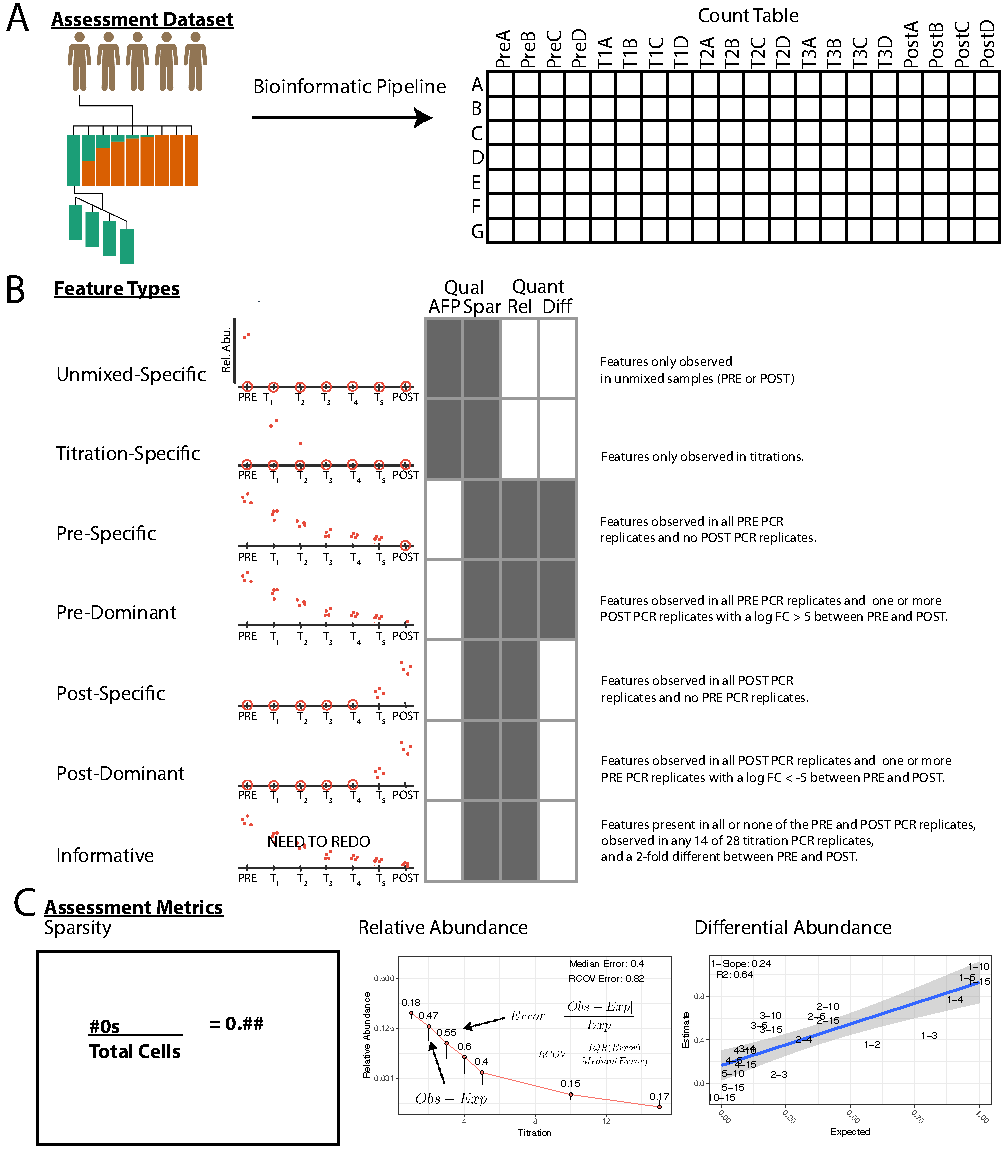
\includegraphics{AssessmentFramework.pdf}
\caption{\label{fig:assessmentFramework}Assessment Framework. (A) Count tables evaluated by the assessment framework are generated from the assessment dataset using marker-gene survey bioinformatic pipelines. Count table rows are features identified by the bioinformatic pipeline and column are samples, four PCR replicates (A-D) for PRE and POST and titrations, to simplify the diagram only three titrations are shown.  The seven features represent the seven feature types observed. (B) Feature type definitions along with pictoral depiction of abundance values and which features are used for the qualitative and quantitative assessments, indicated by grey filled cells in table. (C) Assessment metrics calculated for example count table and example features.}
\end{figure}

Our framework assesses the qualitative and quantitative characteristics of the 16S rRNA measurement process (Fig. \ref{fig:assessmentFramework}).
The framework evaluates count tables generated by bioinformatic pipelines from a data set developed specifically for use in this framework.
The qualitative assessment provides insight into how much confidence a user can have in the presence or absence of a feature, whereas the quantitative assessment evaluates feature abundance values. 
The quantitative assessment evaluates the bias and variance of relative and differential abundance estimates.

\begin{figure}
\centering
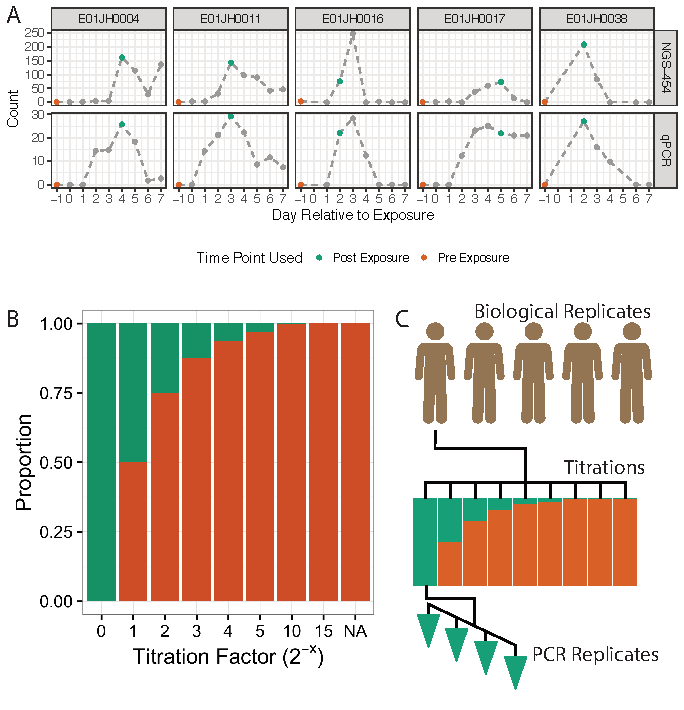
\includegraphics{experimentalDesign.pdf}
\caption{\label{fig:countExperimentalDesign}Sample selection and
experimental design for the two-sample titration 16S rRNA
marker-gene-survey assessment data set. A) Pre- and post-exposure (PRE
and POST) samples from five vaccine trial participants were selected
based on \textit{Escherichia coli} abundance measured using qPCR and 454
16S rRNA sequencing (454-NGS), data from Pop et al. \cite{pop2016individual}.
Counts represent normalized relative abundance values for 454-NGS and
copies of the heat-labile toxin gene per \(\mu L\), a marker gene for
ETEC, for qPCR. PRE and POST samples are indicated with orange and green
data points, respectively. Grey points are other samples from the
vaccine trial time series. B) Proportion of DNA from PRE and POST
samples in titration series samples. PRE samples were titrated into POST
samples following a \(log_2\) dilution series. The NA titration factor
represents the unmixed PRE sample. C) PRE and POST samples from the five
vaccine trial participants, subjects, were used to generate independent
two-sample titration series. The result was a total of 45 samples, 7
titrations + 2 unmixed samples times 5 subjects. Four replicate PCRs
were performed for each of the 45 samples resulting in 190 PCRs.}
\end{figure}

\subsubsection*{Assessment Dataset - Mixture Design}

Using mixtures of environmental samples we generated a data set with expected values for use in our assessment framework. For mixture data sets expected values can be obtained using information from unmixed samples and the mixture design.
Our mixture dataset follows a two-sample titration mixture design, where DNA collected from five vaccine trial participants before and
after exposure to pathogenic \emph{Escherichia coli} was mixed following a \(log_2\) dilution series (Fig. \ref{fig:countExperimentalDesign}). 
For more robust abundance estimates four replicate PCRs assays were performed on each each titration series sample. Throughout the rest of the manuscript samples collected prior to and after \emph{E. coli} exposure are referred to as PRE and POST respectively. 
For our two-sample titration mixture design, the expected feature
relative abundance is calculated using equation \eqref{eq:mixEq},
where \(\theta_i\), is the proportion of POST DNA in titration \(i\),
\(q_{ij}\) is the relative abundance of feature \(j\) in titration
\(i\), and the relative abundance of feature \(j\) in the unmixed PRE
and POST samples is \(q_{pre,j}\) and \(q_{post,j}\).

\begin{equation}
  q_{ij} = \theta_i q_{post,j} + (1 - \theta_i) q_{pre,j}
  \label{eq:mixEq}
\end{equation}

\subsubsection*{Qualitative Assessment}

\begin{figure}
\centering
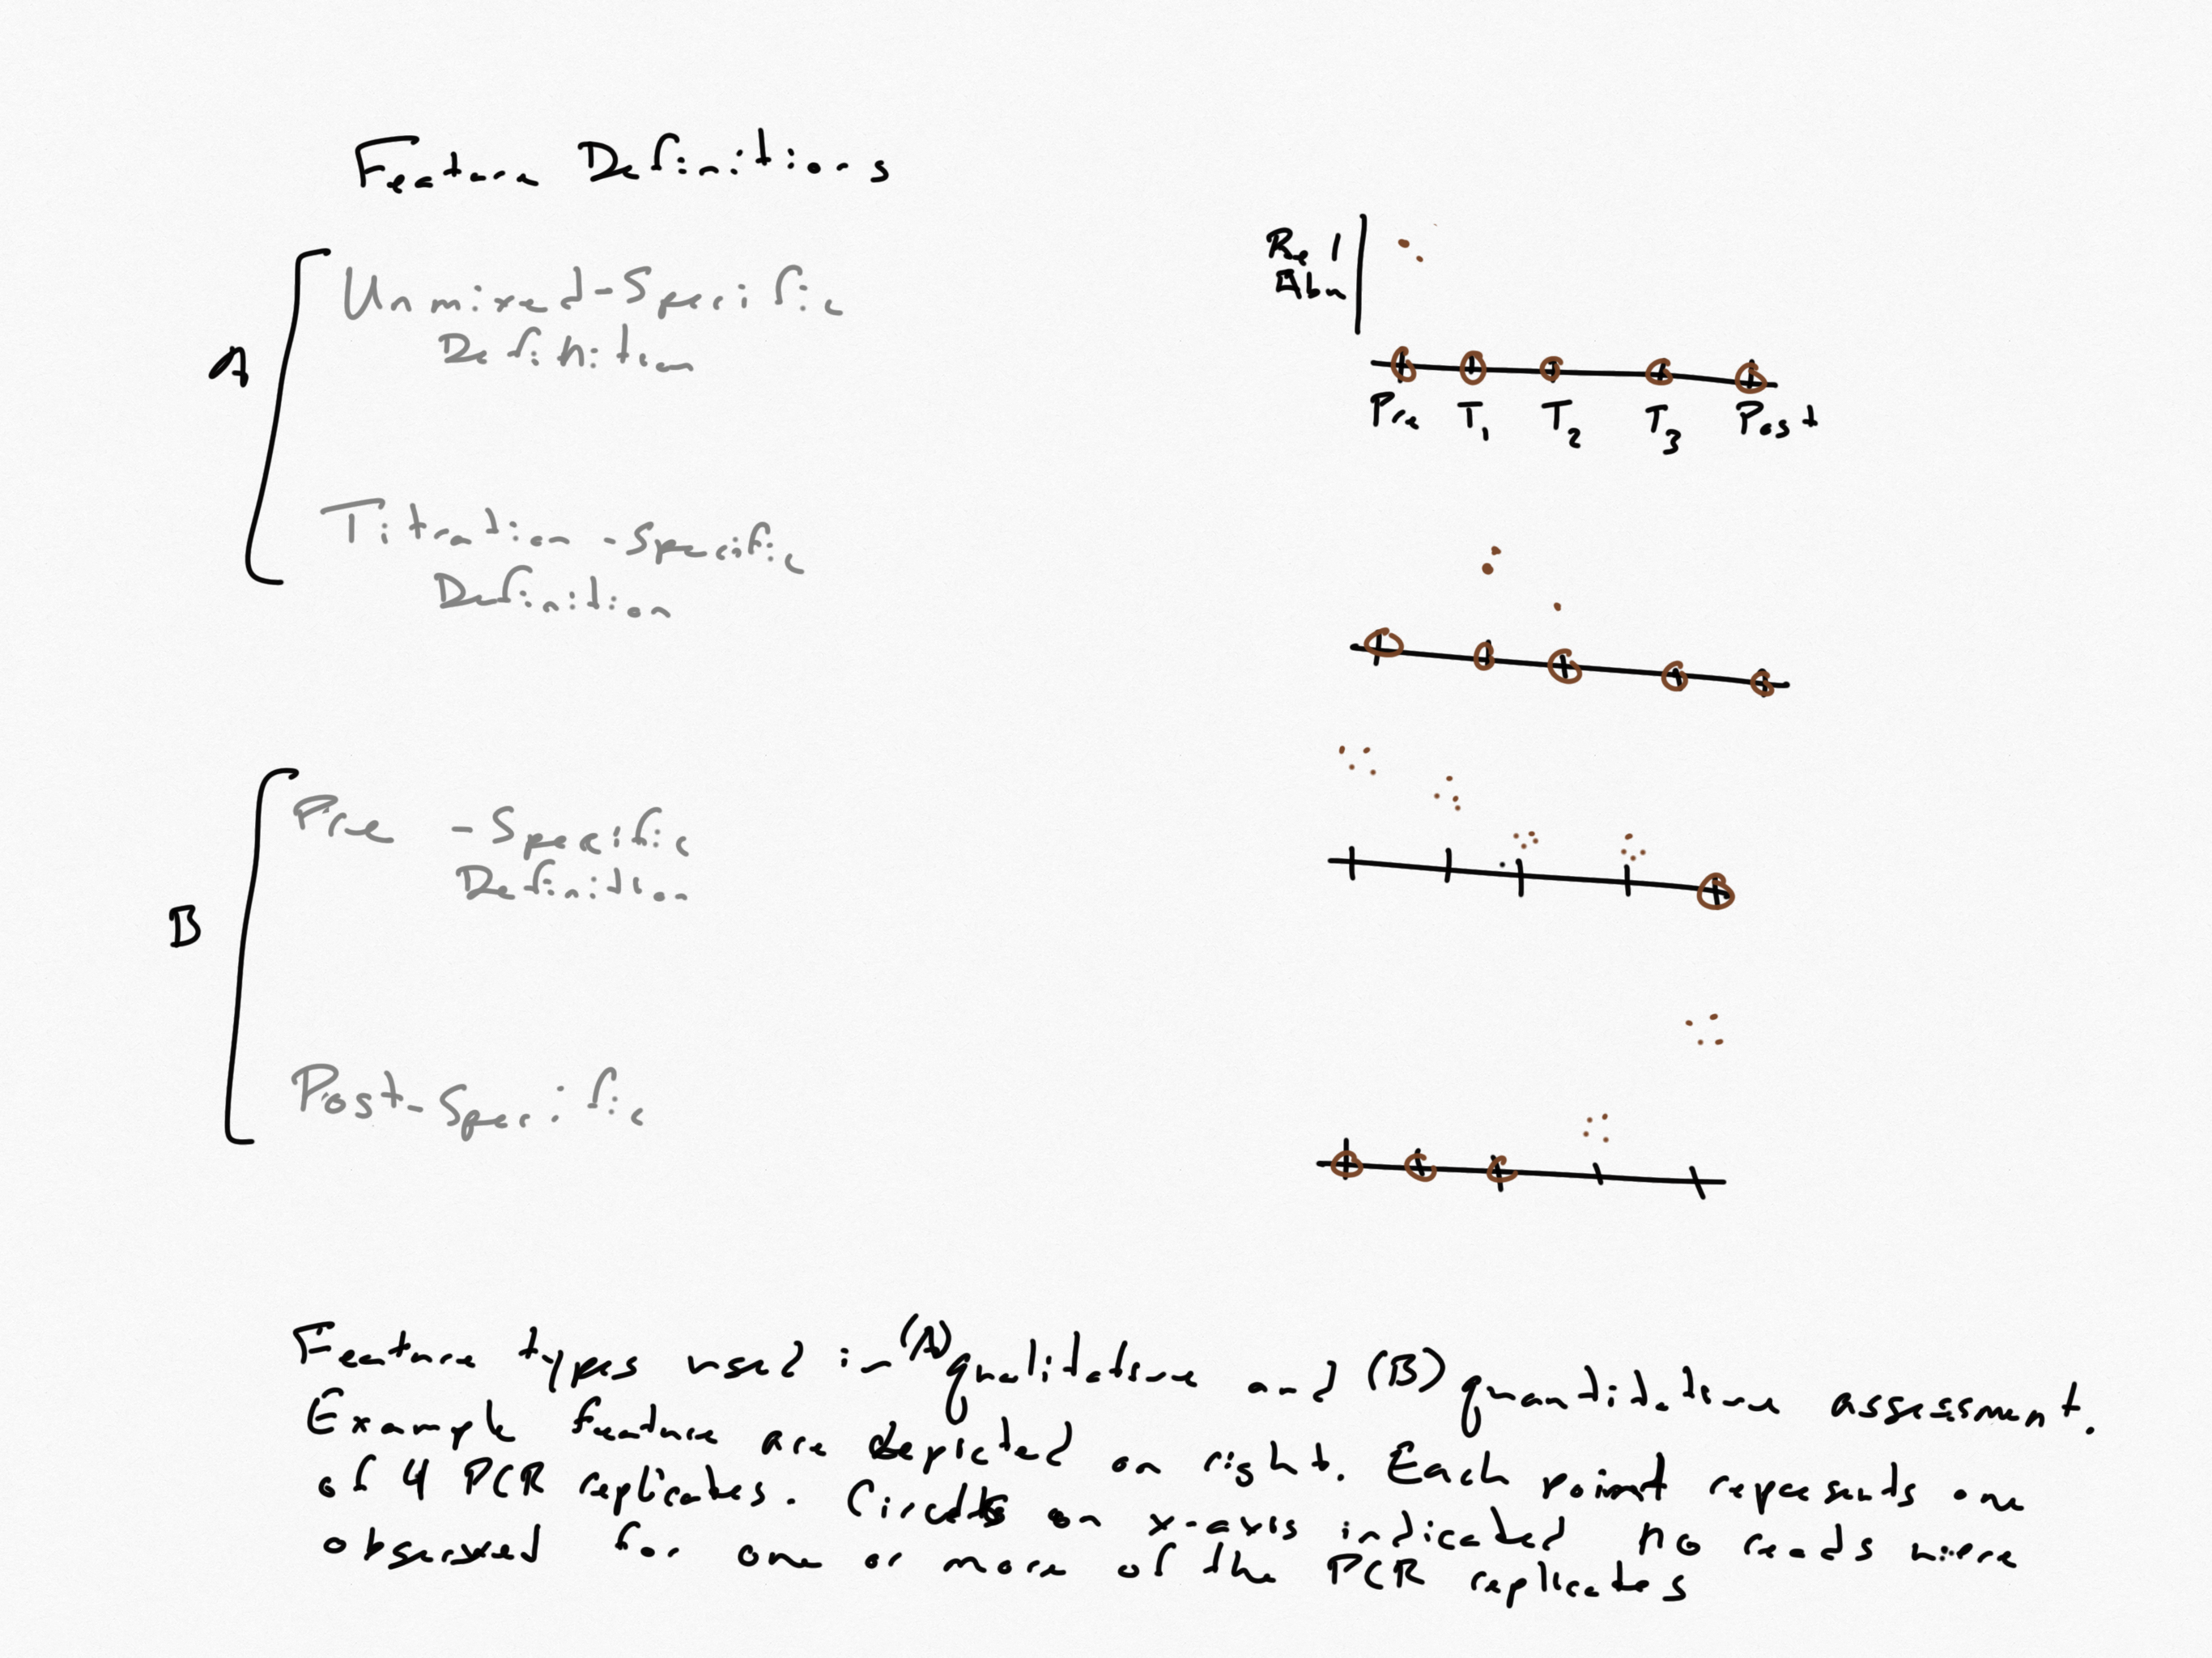
\includegraphics{feature_definitions.png}
\caption{\label{fig:featureDefinitions} Feature types used in (A) qualitative and (B) quantitative assessment. Example features are depicted on right. Each point represents abundance value for one of four PCR replicates. Circles on x-axis indicates no reads observed for one or more of the PCR replicates.}
\end{figure}

The purpose of the qualitative assessment is to show how well pipelines are able to differentiate true biological sequences from measurement process artifacts.
Inadequate processing of artifacts can result in false positive features and false negative features. 
Where false positive features are defined as features present in the count table that are not present in the sequenced sample and false negative features are missing from the count table but present in the biological sample.
Our qualitative assessment methods characterize the artifactual feature proportion, frequency of artifacts in a count table by estimating the proportion of titration-specific and unmixed-specific features (Fig. \ref{fig:featureDefinitions}A) that cannot be explained by sampling alone.
We can combine the artifactual feature proportion assessment results with sparsity estimates to determine whether the artifacts are primarily false positives or negatives.
Sparsity is defined as the fraction of 0 valued cells in a matrix, here count tables.
%% Make sure these definitions are consistent with rest of text - do these make sense - how to address ambiguity in how these can be defined.
%Here we will define a false positive as a feature present in a titration but not observed in the unmixed samples, %titration-specific, and false negative as features observed in unmixed samples but not the titrations, unmixed-specific.

%% This definition is DADA2 specific ...
The artifactual feature proportion assessment evaluates whether titration- and unmixed-specific features can be explained by sampling alone.
Features present only in titrations or unmixed samples not due to random
sampling are measurement process artifacts. These artifacts can be
categorized as false negative or false positive features. A false
negative occurs when a lower abundance sequence representing an organism
within the sample is clustered with a higher abundance sequence from a
different organism. 
%% Can also occur when a feature is not amplified
False positives are sequencing or PCR artifacts not
appropriately filtered or correctly assigned to a feature by the
bioinformatic pipeline.
False positive and negative features can result in artificially inflated or deflated diversity estimates.

%% Add diagram for sparsity and artifactual features

\subsubsection*{Quantitative Assessment}

\begin{figure}
\centering
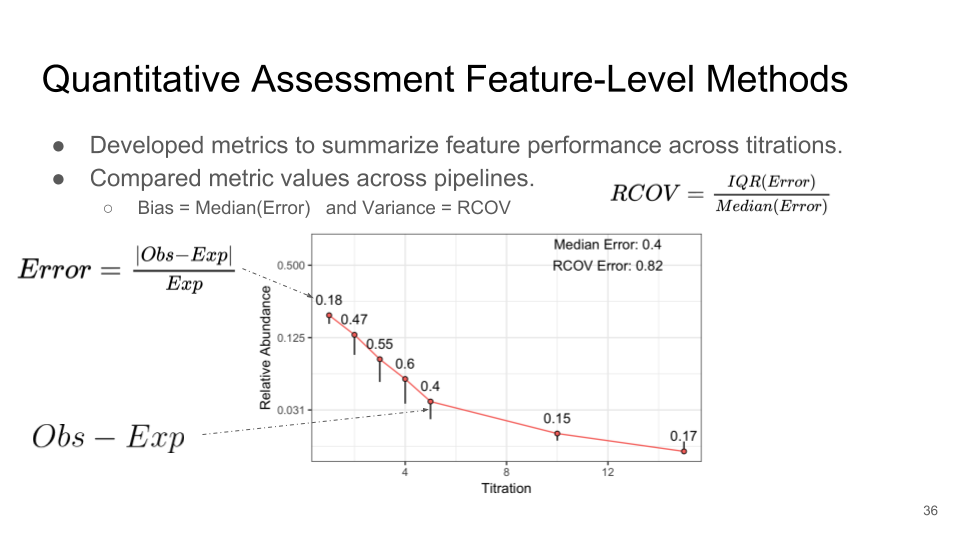
\includegraphics{quant_metrics.png}
\caption{\label{fig:quantMetrics} Quantitative metrics diagram.}
\end{figure}

To evaluate count table abundance values our quantitative assessment uses error, bias, and variance metrics (Fig. \ref{fig:quantMetrics}).
The error metrics measure agreement between observed and expected values for individual replicates.
The bias and variance metrics are a measure of feature-level performance.
Metric distributions are used to evaluate overall pipeline performance by providing insight into overall trends. 
For example precise and not accurate abundance estimates have skewed error metrics with a narrow distribution.
Additionally, feature-level metrics can be used to identify feature-specific biases. 


\paragraph*{Relative Abundance Assessment}
%% Move to methods?? or theta correction section
%The PRE and POST
%estimated relative abundance and \(\theta\) values were used to
%calculate titration and relative abundance error rates. 

Relative abundance error rate is defined as \(|exp - obs|/exp\), where \(exp\)
and \(obs\) is the expected and observed relative abundance.


ADD TEXT - bias and variance metric definitions

\paragraph*{Differential Abundance Assessment}
ADD TEXT - metric definitions

\subsection*{Assessment Data set Characterization and Validation}
%% This statement needs work
To assure the dataset is suitable for use in our assessment framework we first validated the titration series and raw sequence data. 
We additionally evaluated the sequence dataset for subject specific differences that would inform the interpretation of our assessment results.

\subsubsection*{Assessment Dataset Characterization}

\begin{figure}
\centering
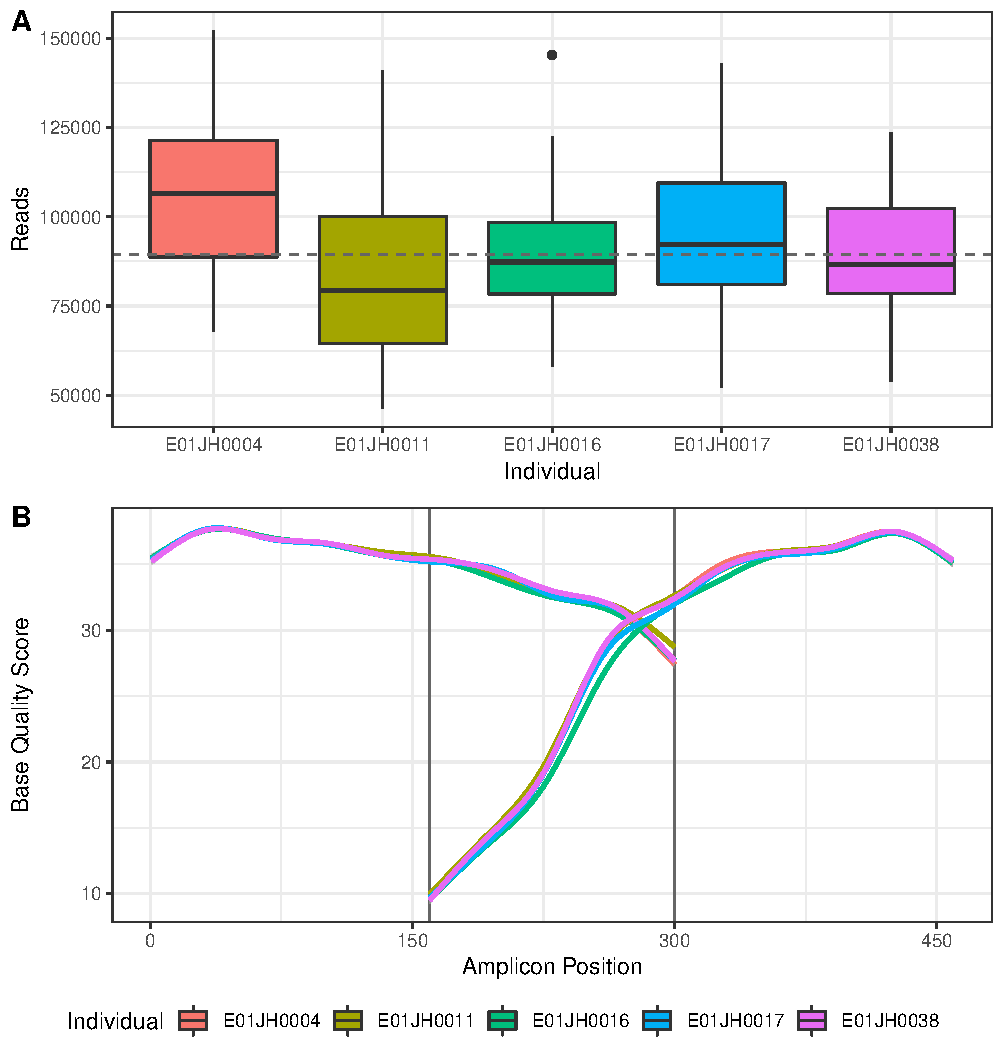
\includegraphics{qaPlots-1.pdf}
\caption{\label{fig:qaPlots}Sequence data set characteristics. (A)
Distribution in the number of raw reads generated per barcoded sample (Library Size)
by individual. Boxplots summarize data distribution with horizontal bar
as median, boxes indicating interquartile range, whiskers
\(\pm 1.5\times IQR\), and black points outliers. The dashed horizontal
line indicates overall median library size. Excluding one PCR replicate
from subject E01JH0016 titration 5 that had only 3,195 reads. (B)
Smoothing spline of the base quality score (BQS) across the amplicon by
subject. Vertical lines indicate approximate overlap region between
forward and reverse reads. Forward reads go from position 0 to 300 and
reverse reads from 464 to 164.}
\end{figure}

To evaluate the overall sequencing data set quality and check for subject
specific differences we characterized the number of reads per sample and
base quality score distribution. The number of reads per sample and
distribution of base quality scores by position was consistent across subjects (Fig. \ref{fig:qaPlots}). 
Two barcoded experimental samples had less than
35,000 reads and are likely the product of failed PCRs.
Therefore, these samples were excluded from downstream analysis.
The rest of the samples with less than 35,000 reads were no template PCR
controls (NTC). Excluding one failed reaction with 2,700 reads and NTCs, there
were \(8.9548\times 10^{4}\) (3195-152267) sequences per sample, median and
range. Forward reads had consistently higher base quality scores relative to
the reverse reads with a narrow overlap region with high base quality scores
for both forward and reverse reads (Fig. \ref{fig:qaPlots}B).
No subject specific differences in read quality were observed.

%% Add subject specific characterization requested by one of the reviewers here.

\subsubsection*{Assessment Dataset Validation}

\begin{figure}
\centering
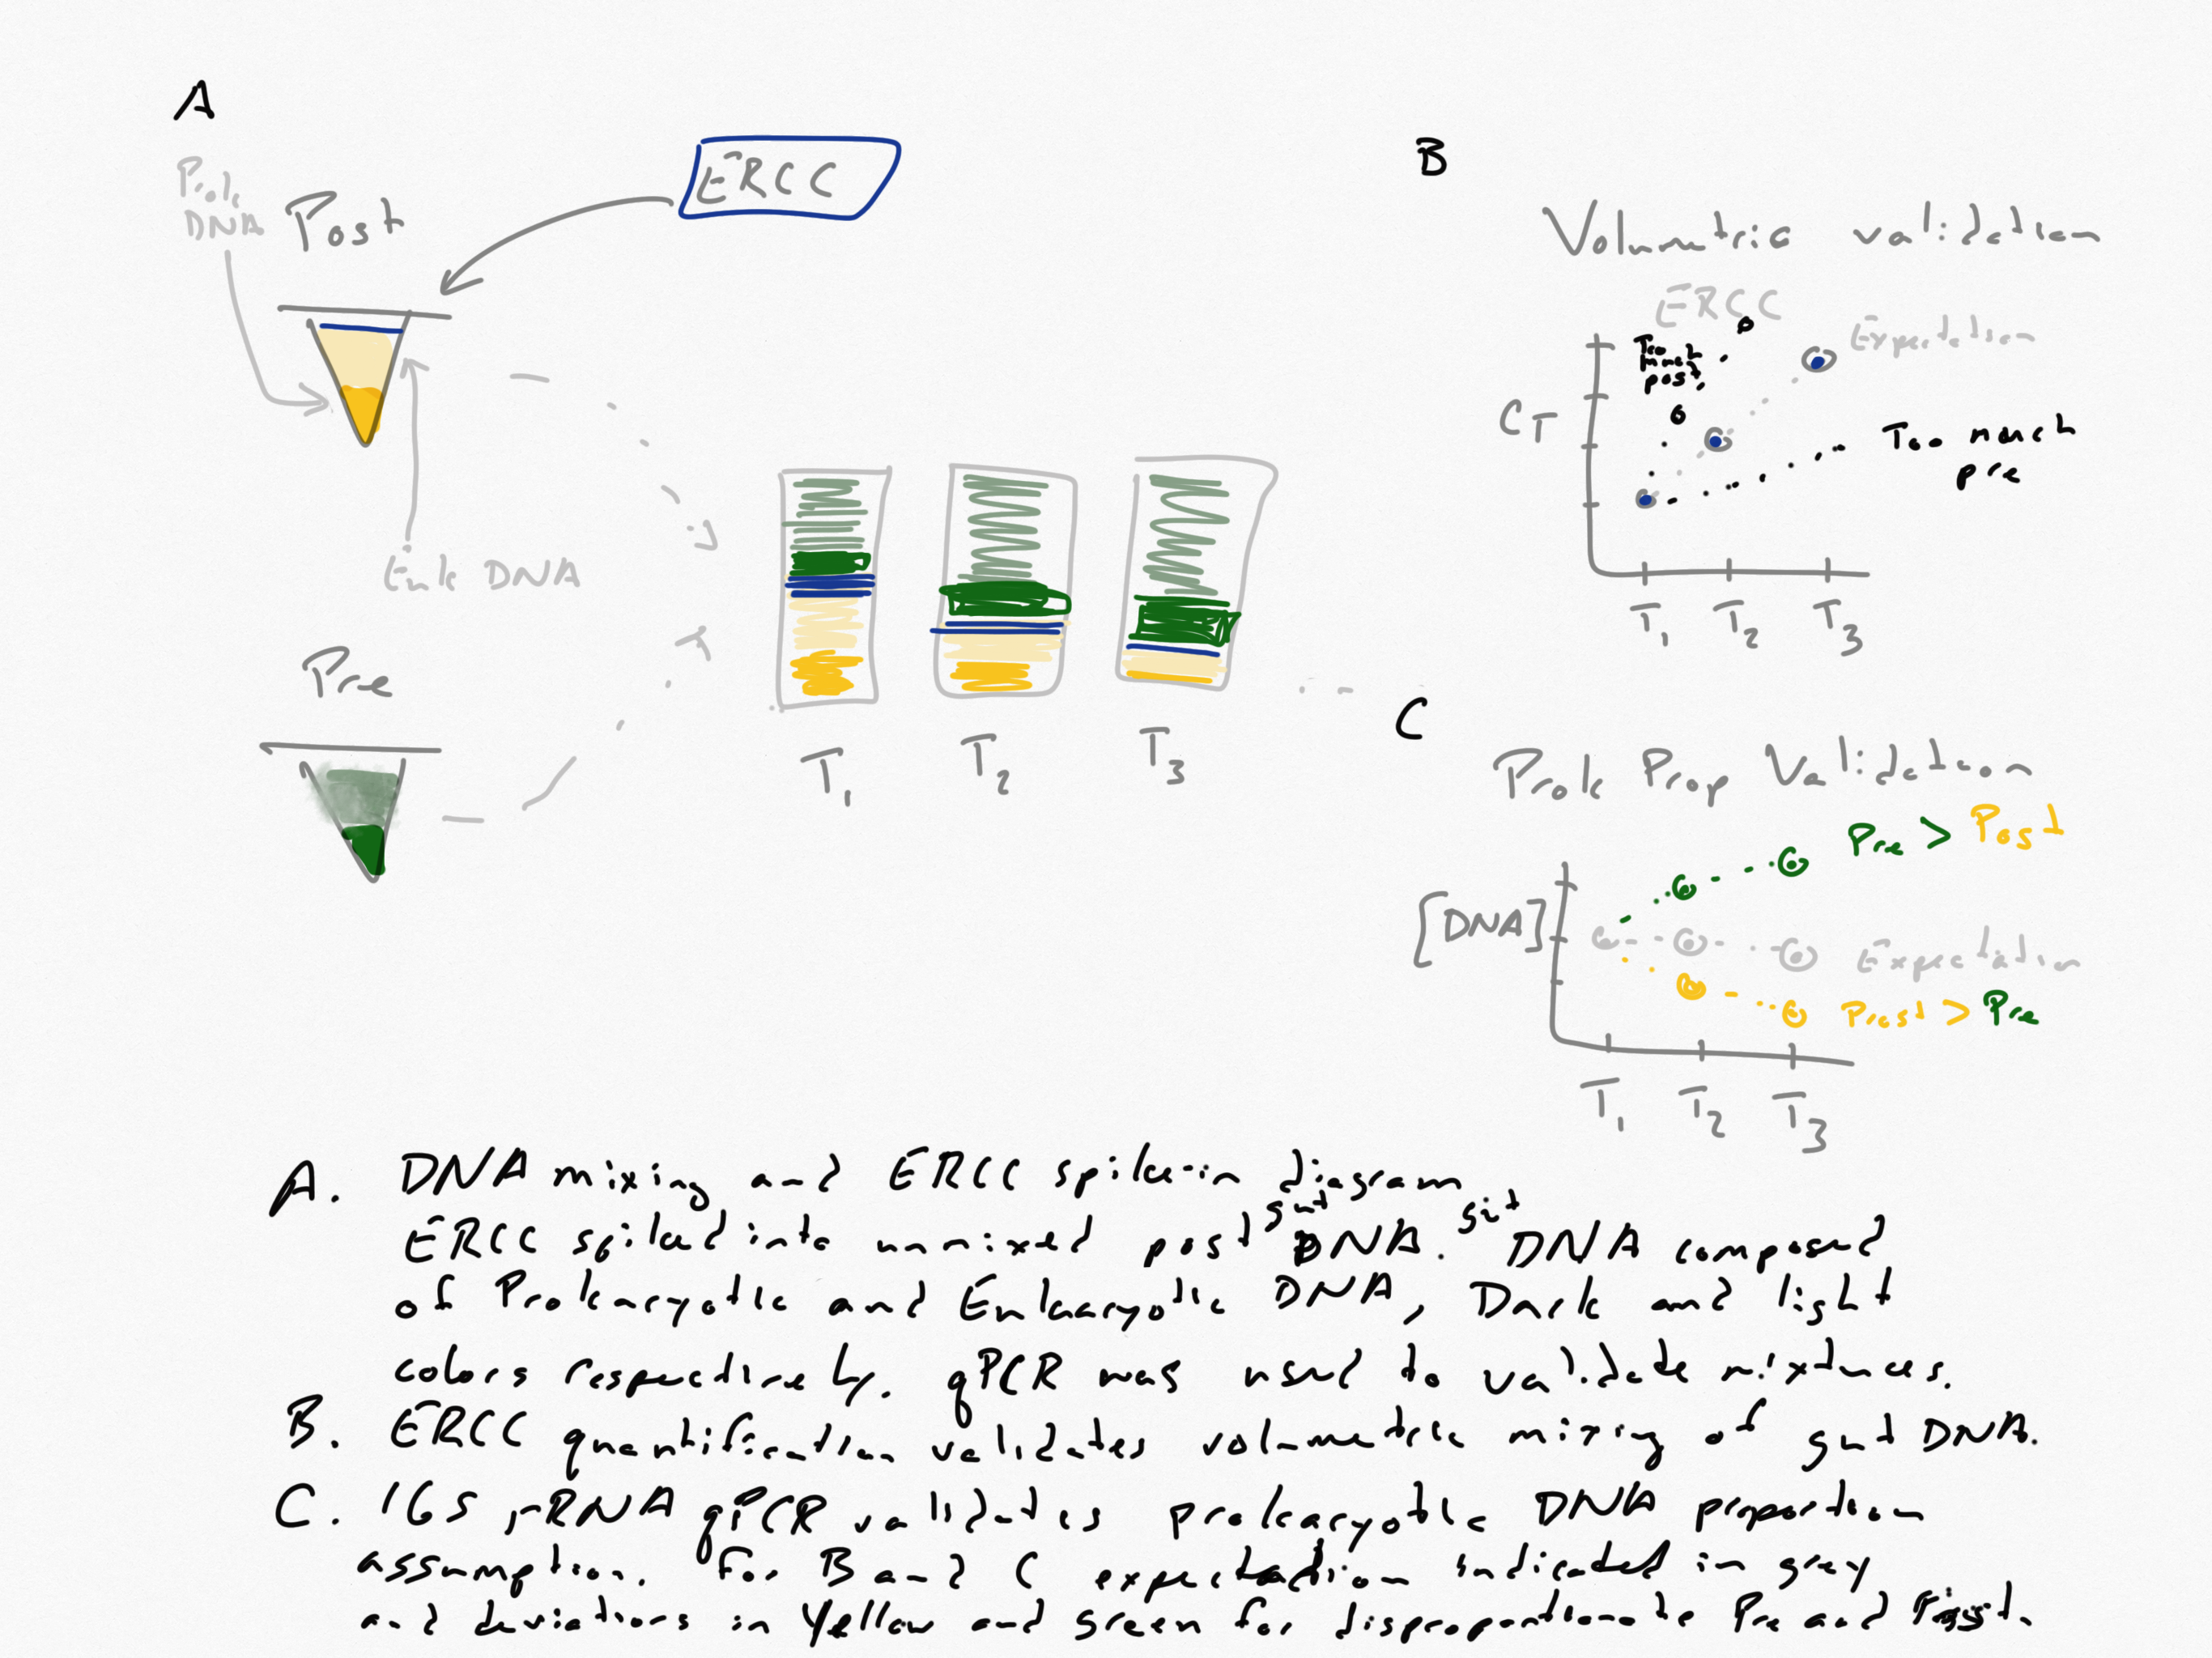
\includegraphics{titration_validation.png}
\caption{\label{fig:titrationValidation} Titration-series validation methods. (A) ERCCs were spiked into unmixed PRE and POST DNA. Unmixed DNA is composed of prokaryotic and eukaryotic DNA. The proportion of prokarytic DNA differs between PRE and POST resulting in the proportion of measureable PRE and POST DNA (prokarytic DNA) in the titrations differing from the mixture design. (B) Results from qPCR quantification of the ERCCs was used to validate volumetric mixing. (C) 16S rRNA qPCR is used to validate the prokaryotic DNA proportion. For B and C expectation is indicated in grey. Deviations from expectation along with explanations are indicated in black for B and yellow and green for C.}
\end{figure}

To validate the two-sample titration dataset for use in our assessment framework 
we evaluated two assumptions about the titrations.
(1) The samples were mixed volumetrically in a
\(log_2\) dilution series according to the mixture design. 
(2) The unmixed PRE and POST samples
have the same proportion of prokaryotic DNA.
To validate the sample volumetric mixing exogenous DNA (ERCC plasmids) were spiked into the
unmixed samples before mixing and quantified
using qPCR (Fig. \ref{fig:titrationValidation}).
The stool samples used to
generate the mixtures have both eukaryotic (primarily human) DNA and
prokaryotic DNA. If the proportion of prokaryotic DNA differs between
the unmixed samples, then the amount of DNA from the unmixed samples in
a titration targeted by 16S rRNA gene sequencing is not consistent with
the mixture design. To evaluate if the PRE and POST samples had the same
proportion of prokaryotic DNA in the titrations
samples were quantified using a qPCR assay targeting the 16S rRNA gene (Fig. \ref{fig:titrationValidation}).


\paragraph*{Volumetric Mixing Validation}

Titration series volumetric mixing was validated using qPCR to quantify exogenous
DNA (ERCC plasmids) spiked into the POST samples prior to mixing.
The expectation is that the ERCC plasmid copy number will change at a rate consistent
with the change in proportion of POST along the titration series (Fig. \ref{fig:countExperimentalDesign}B and \ref{fig:titrationValidation}).
For our \(log_2\) two-sample-titration mixture design the expected slope of the
regression line between titration factor and Ct is 1, corresponding to a
doubling in template DNA every PCR cycle. The qPCR assay
standard curves had a high level of precision with \(R^2\) values close
to 1 and amplification efficiencies between 0.84 and 0.9 for all
standard curves indicating the assays were suitable for validating the
titration series volumetric mixing (Table \ref{tab:erccTable}). The qPCR assays targeting the
ERCCs spiked into the POST samples had \(R^2\) values and slope
estimates close to 1 (Table \ref{tab:erccTable}). Slope estimates less
than one were attributed to assay standard curve efficiency less than 1
(Table \ref{tab:erccTable}). When considering the
quantitative limitations of the qPCR assay these results confirm that
the unmixed samples were volumetrically mixed according to the
two-sample titration mixture design.

\begin{table}

\caption{\label{tab:erccTable}ERCC Spike-in qPCR assay information and summary statistics. ERCC is the ERCC identifier for the ERCC spike-in, Assay is TaqMan assay, and Length and GC are the size and GC content of the qPCR amplicon.  The Std. $R^2$ and Efficiency (E) statistics were computed for the standard curves. $R^2$ and slope for titration qPCR results for the titration series.}
\centering
\begin{tabular}[t]{lllrrrrr}
\toprule
Subject & ERCC & Assay & Length & Std. $R^2$ & E & $R^2$ & Slope\\
\midrule
E01JH0004 & 012 & Ac03459877-a1 & 77 & 0.9996 & 86.19 & 0.98 & 0.92\\
E01JH0011 & 157 & Ac03459958-a1 & 71 & 0.9995 & 87.46 & 0.95 & 0.90\\
E01JH0016 & 108 & Ac03460028-a1 & 74 & 0.9991 & 87.33 & 0.95 & 0.84\\
E01JH0017 & 002 & Ac03459872-a1 & 69 & 0.9968 & 85.80 & 0.89 & 0.93\\
E01JH0038 & 035 & Ac03459892-a1 & 65 & 0.9984 & 86.69 & 0.95 & 0.94\\
\bottomrule
\end{tabular}
\end{table}


\begin{figure}
\centering
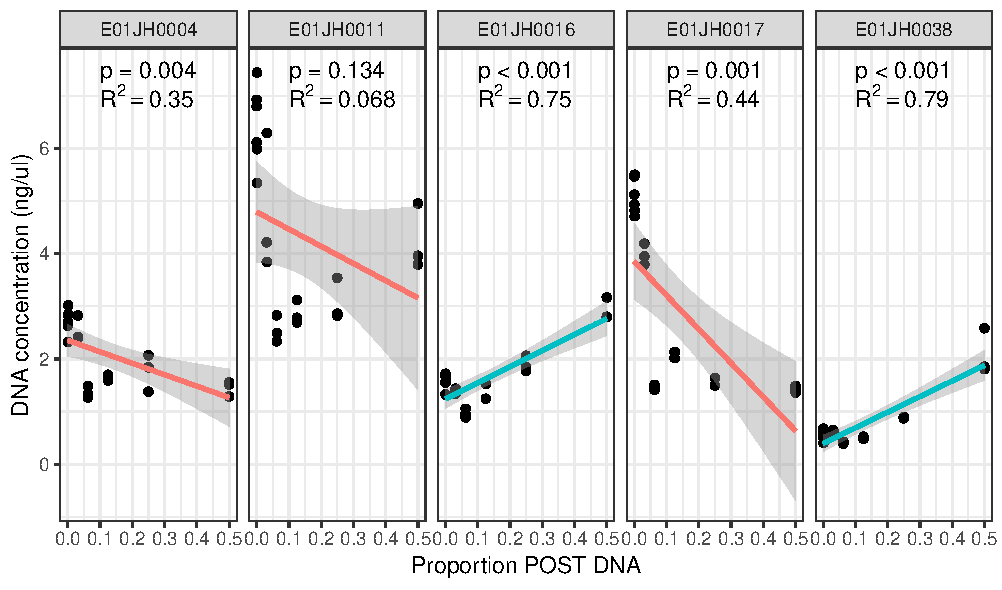
\includegraphics{bacPlot-1.pdf}
\caption{\label{fig:bacPlot}Prokaryotic DNA concentration (ng/ul) across
titrations measured using a 16S rRNA qPCR assay. \(R^2\) and p-values are linear models fit to prokaryotic DNA concentration versus proportion post DNA for each individual.
Red and blue lines indicate negative and positive slope estimates respectively.
p-value indicates significant difference from the expected slope of 0.
The grey regions indicate the linear model 95\% confidence interval.
Multiple test correction was performed using the Benjamini-Hochberg
method. One of the E01JH0004 PCR replicates for titration 3
(\(\theta=0.125\)) was identified as an outlier, with a prokaryotic DNA
concentration of 0.003 ng/ul, and was excluded from the linear model.
The linear model slope was still significantly different from 0 when the
outlier was included.}
\end{figure}

\paragraph*{Prokaryotic DNA Proportion Validation}
Observed changes in prokaryotic DNA concentration across titrations
indicate the proportion of prokaryotic DNA from the unmixed PRE and POST
samples in a titration is inconsistent with the mixture design (Fig.
\ref{fig:bacPlot}). A qPCR assay targeting the 16S rRNA gene was used to
quantify the concentration of prokaryotic DNA in the titrations. If the
proportion of prokaryotic DNA is the same between PRE and POST samples
the slope of the concentration estimates across the two-sample titration
would be 0. For subjects where the proportion of prokaryotic DNA is
higher in the PRE samples, the slope will be negative, and positive when
the proportion is higher for POST samples. The slope estimates are
significantly different from 0 for all subjects excluding E01JH0011
(Fig. \ref{fig:bacPlot}). These results indicate that the proportion of
prokaryotic DNA is lower in POST when compared to the PRE samples for
E01JH0004 and E01JH0017 and higher for E01JH0016 and E01JH0038.





%% Need to include bioinformatic pipeline information

\paragraph*{Correcting for Deviations from Mixture Design}
%% Incorporate into text - only present unclustered
% The unclustered count table was generated using the
% 40,000 most abundant features from Mothur's initial pre-processing (see
% Methods for details).
% Unclustered pipeline \(\theta\) estimates were
% used to calculate the error rates for all pipelines to prevent
% over-fitting.


Our titration validation results identified differences in the proportion of prokaryotic DNA in PRE and POST samples (Fig. \ref{fig:bacPlot}).
Therefore our expected values used in measurement assessment need to account for differences in the proportion of prokaryotic DNA from unmixed samples.
To account for differences in prokaryotic DNA proportion we inferred
the proportion of POST sample prokaryotic DNA in a titration, \(\theta\), using
the 16S rRNA sequencing data (Fig. \ref{fig:thetaHat}). Overall the relationship
between the inferred and mixture design \(\theta\) values were
consistent across pipelines but not subject whereas the \(\theta\)
estimate 95\% CI varied by both subject and pipeline. For study subjects
E01JH0004, E01JH0011, and E01JH0016 the inferred and mixture design
\(\theta\) values were in agreement, in contrast to study subjects
E01JH0017 and E01JH0038. For E01JH0017 the inferred values were
consistently less than the mixture design values. For E01JH0038
the inferred values were consistently greater than the mixture design
values. These results were consistent with the qPCR prokaryotic DNA
concentration results with significantly positive slopes for E01JH0004
and E01JH0016 and significantly negative slope for E01JH0038 (Fig.
\ref{fig:bacPlot}).

\begin{figure}
\centering
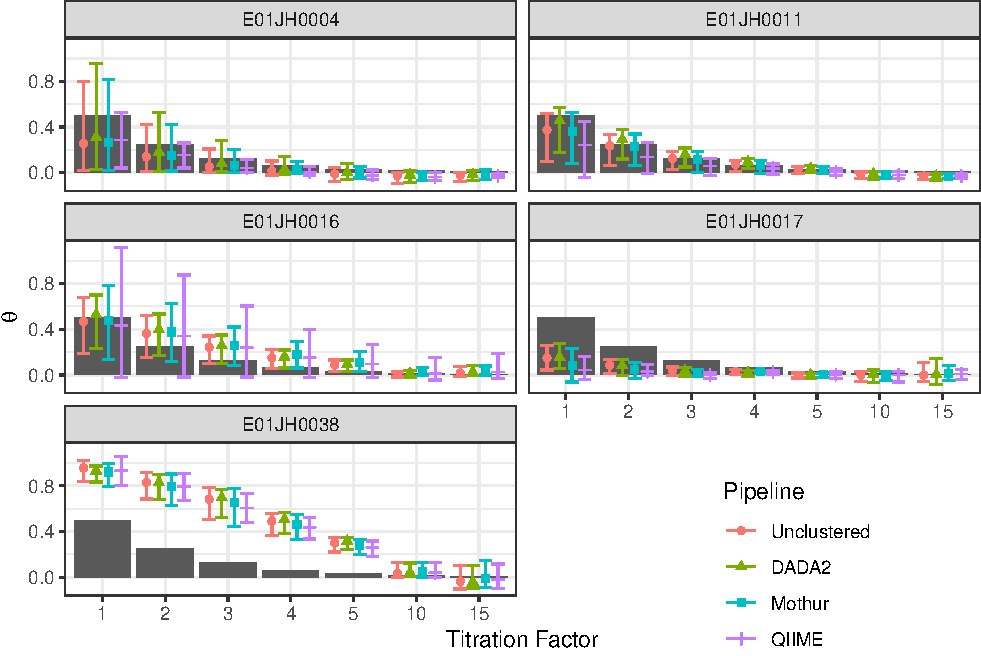
\includegraphics{thetaHat-1.pdf}
\caption{\label{fig:thetaHat}Theta estimates (\(\hat{\theta}\)) by titration, biological
replicate, and bioinformatic pipeline. Points indicate mean
of 1000 bootstrap \(\theta\) estimates and error bars 95\% confidence
interval. Grey bars indicate expected \(\theta\) values based on mixture design.
Points above grey bars indicate the titrations with a high proportion of prokaryotic DNA from the POST sample than expected. Points below grey bars indicate titrations with high proportion of prokaryotic DNA from the PRE sample.}
\end{figure}


\subsection*{Count Table Assessment Demonstration}
Next, we demonstrate our assessment framework on count tables generated using
three different bioinformatic pipelines; 
DADA2, a denoising sequence inference pipeline; 
QIIME, an open-reference clustering pipeline; 
and Mothur, a de-novo clustering pipeline. 
To provide insight into how the three count tables are quantitatively different we first provide high level summary statistics. 
Next we will compare the results from applying our assessment framework to three count tables.

\paragraph{Count Table Characteristics}
\begin{table}
\caption{\label{tab:pipeQA}Summary statistics for the different bioinformatic pipelines. DADA2 is a denoising sequence inference pipeline, QIIME is an open-reference clustering pipeline, and Mothur  is a de-novo clustering pipeline. No template controls were excluded from summary statistics. Sparsity is the proportion of 0's in the count table. Features is the total number of OTUs (QIIME and Mothur ) or SVs (DADA2) in the count. Sample coverage is the median and range (minimum-maximum) per sample total abundance. Drop-out rate is the proportion of reads removed while processing the sequencing data for each bioinformatic pipeline.}
\centering
\begin{tabular}[t]{lrrll}
\toprule
Pipelines & Features & Sparsity & Total Abundance & Drop-out Rate\\
\midrule
DADA2 & 3144 & 0.93 & 68649 (1661-112058) & 0.24 (0.18-0.59)\\
Mothur & 38358 & 0.98 & 53775 (1265-87806) & 0.4 (0.35-0.62)\\
QIIME & 11385 & 0.94 & 25254 (517-46897) & 0.7 (0.62-0.97)\\
\bottomrule
\end{tabular}
\end{table}

\begin{figure}
\centering
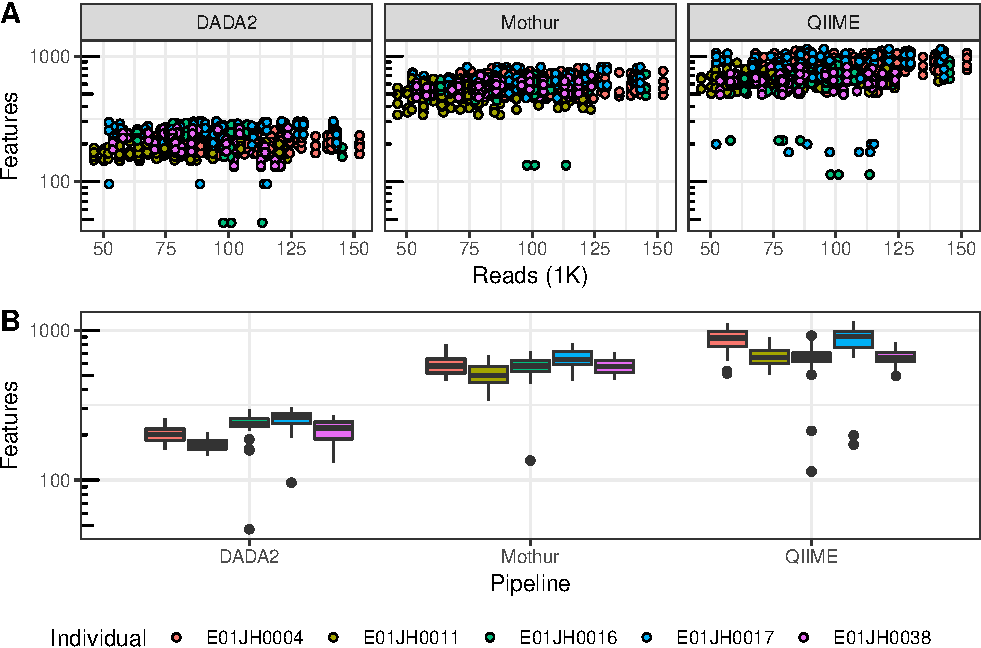
\includegraphics{readsVfeats-1.pdf}
\caption{\label{fig:readsVfeats}Relationship between the number of reads and
features per sample by bioinformatic pipeline. (A) Scatter plot of
observed features versus total abundance per sample. (B) Observed
feature distribution by pipeline and individual. Excluding one PCR
replicate from subject E01JH0016 titration 5 with only 3,195 reads, and
the Mothur E01JH0017 titration 4 (all four PCR replicates), with 1,777
observed features.}
\end{figure}

\begin{figure}
\centering
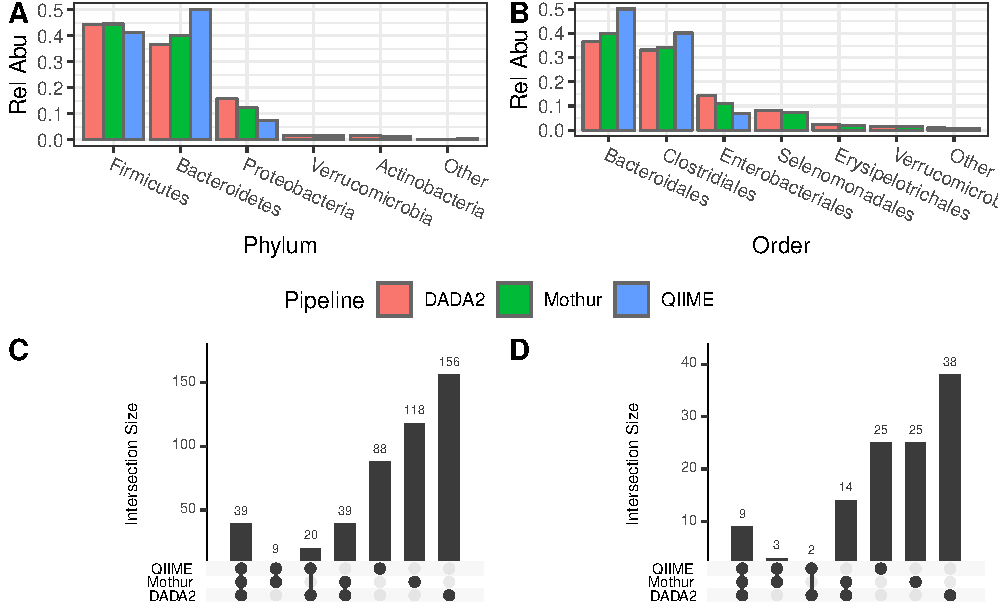
\includegraphics{pipeTaxa-1.pdf}
\caption{\label{fig:pipeTaxa}Comparison of dataset taxonomic composition
across pipelines. Phylum (A) and Order (B) relative abundance by
pipeline. Taxonomic groups with less than 1\% total relative abundance
were grouped together and indicated as other. Pipeline genus-level
taxonomic assignment set overlap for all genera (C) and the upper
quartile genera by relative abundance for each pipeline (D). Intersection size is the number of features observed in the pipeline combination indicated on the x-axis. For example in C, 39 genera are observed in all three pipelines and 88 are observed in only QIIME and not Mothur or DADA2.}
\end{figure}

The count tables generated using the three bioinformatic pipelines vary in pre-processing and feature inference methods. These differences are reflected in the count table number of features, total abundance, and filter rate (Table \ref{tab:pipeQA}, Figs. \ref{fig:readsVfeats}B). The
pipelines evaluated employ different approaches for handling low quality
reads resulting in large differences in filter rate and the fraction
of raw sequences not included in the count table (Table
\ref{tab:pipeQA}). QIIME pipeline has the highest filter rate and
number of features per sample but fewer total features than Mothur. The
targeted amplicon region has a relatively small overlap region, 136 bp
for 300 bp paired-end reads, compared to other commonly used amplicons
\cite{kozich2013development, Walters2016-lf}. The high filter rate is
due to low basecall accuracy at the ends of the reads especially the
reverse reads resulting in a high proportion of unsuccessfully merged
reads pairs (Fig. \ref{fig:qaPlots}B). Further increasing the
filter rate, QIIME excludes singletons, features only observed once in
the data set. 

%% Include motivation statement
Data set taxonomic assignments also varied by pipeline (Fig.
\ref{fig:pipeTaxa}). Phylum and order relative abundance is similar
across pipelines (Fig. \ref{fig:pipeTaxa}A \& B). The observed
differences are attributed to different taxonomic classification methods
and databases used by the pipelines. DADA2 and QIIME pipelines differed
from Mothur and QIIME for Proteobacteria and Bacteriodetes. Regardless
of the relative abundance threshold, for genus sets most genera were
unique to individual pipelines (Fig. \ref{fig:pipeTaxa}C \& D). Sets,
shared taxa between pipelines, with QIIME had the fewest genera,
excluding the DADA2-QIIME set. QIIME was the only pipeline to use
open-reference clustering and the Greengenes database. Mothur and DADA2
both used the SILVA dataset. The Mothur and DADA2 pipeline use different
implentations of the RDP naïve Bayesian classifier, which may be
partially responsible for the Mothur, unclustered, and DADA2
differences.

\subsubsection*{Qualitative Assessment}

\begin{figure}
\centering
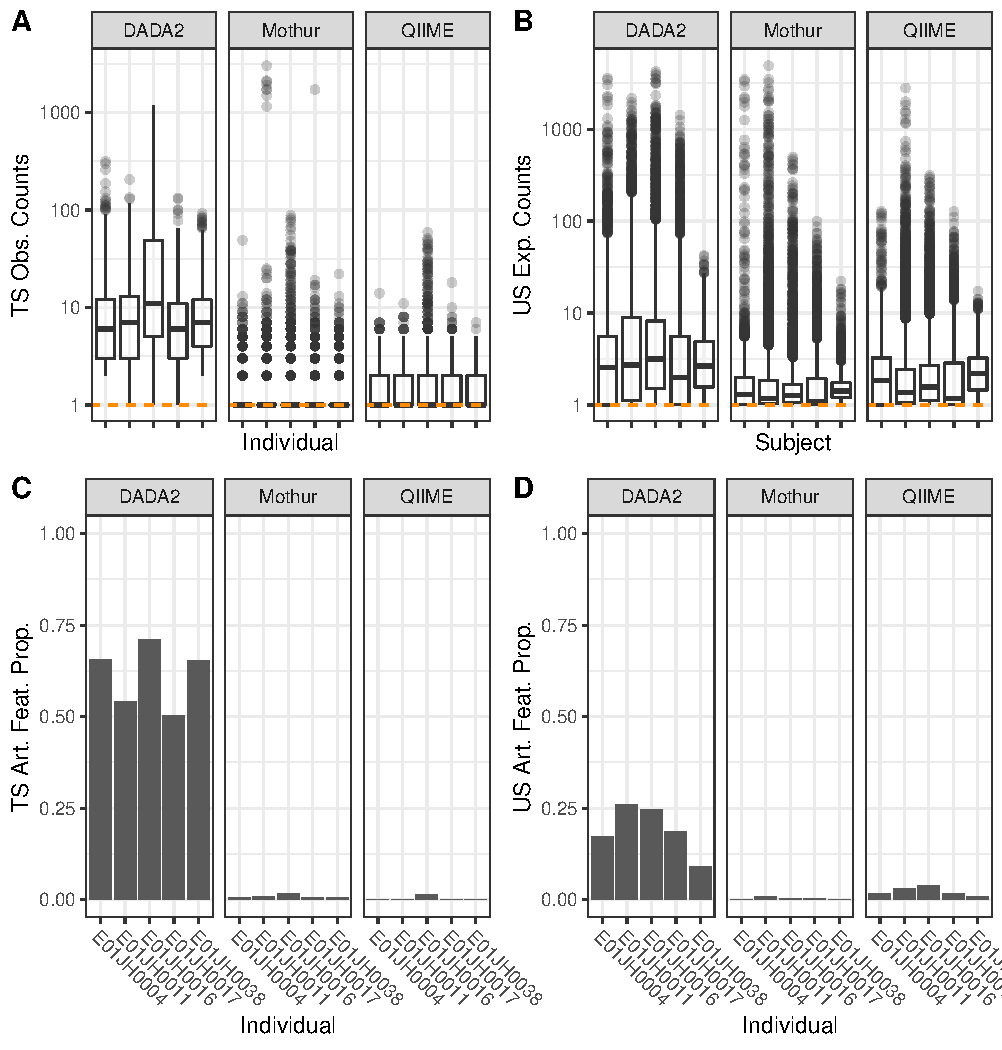
\includegraphics{qualPlot-1.pdf}
\caption{\label{fig:qualPlot}Distribution of (A) observed count values for
titration-specific features and (B) expected count values for
unmixed-specific features by pipeline and individual. The orange
horizontal dashed line indicates a count value of 1. (C) Proportion of
unmix-specific features and (D) titration-specific features with an
adjusted p-value \textless{} 0.05 for the Bayesian hypothesis test and
binomial test respectively. We failed to accept the null hypothesis when
the p-value \textless{} 0.05, indicating that the discrepancy between
the feature only being observed in the titrations or unmixed samples
cannot be explained by sampling alone.}
\end{figure}

The evaluate feature presence-absence the qualitative assessment measures the artifactual feature proportion and uses sparsity to interpret the results. 
DADA2 had a higher artifactual feature proportion relative to the other pipelines with DADA2 and QIIME being similarly sparse and Mothur was a little less sparse.
Unmixed- and titration-specific features were observed for all pipelines
(titration-specific: Fig. \ref{fig:qualPlot}A, unmixed-specific: Fig.
\ref{fig:qualPlot}B).
For mixture datasets, low abundance features
present only in unmixed samples and mixtures are expected due to random
sampling. For our two-sample titration dataset, there were
unmixed-specific features with expected counts not explained by sampling
alone for all individuals and bioinformatic pipelines (Fig.
\ref{fig:qualPlot}C). However, the proportion of unmixed-specific
features that could not be explained by sampling alone varied by
bioinformatic pipeline. DADA2 had the highest proportion of
unmixed-specific features not explained by sampling whereas QIIME had
the lowest proportion which is consistent with the distribution of titration-specific feature observed
counts (Fig.
\ref{fig:qualPlot}D). Overall, the DADA2 count table had the largest
number of observed features inconsistent with the titration experiment
design, while the same phenomenon is significantly reduced in the other
pipelines.

%% Relate to artifactual feature proportion
% Both features explained by sampling and not effect sparsity - can calculate sparsity excluding features that could be explained by sampling. Change in values indicator of long population tail
Despite the differences in total abundance and number of features
the count tables generated using the three bioinformatic pipelines were
similarly sparse (Table \ref{tab:pipeQA}).
The expectation is that this mixture dataset will be
less sparse relative to other datasets. 
This is due to the redundant
nature of the samples where the 35 titration samples are derived
directly from the 10 unmixed samples, along with four PCR replicates for
each sample. With sparsity greater than 0.9 for the three pipelines it
is unlikely that any of the pipelines successfully filtered out a
majority of the sequencing artifacts.


\subsubsection*{Quantitative Assessment}

\begin{figure}
\centering
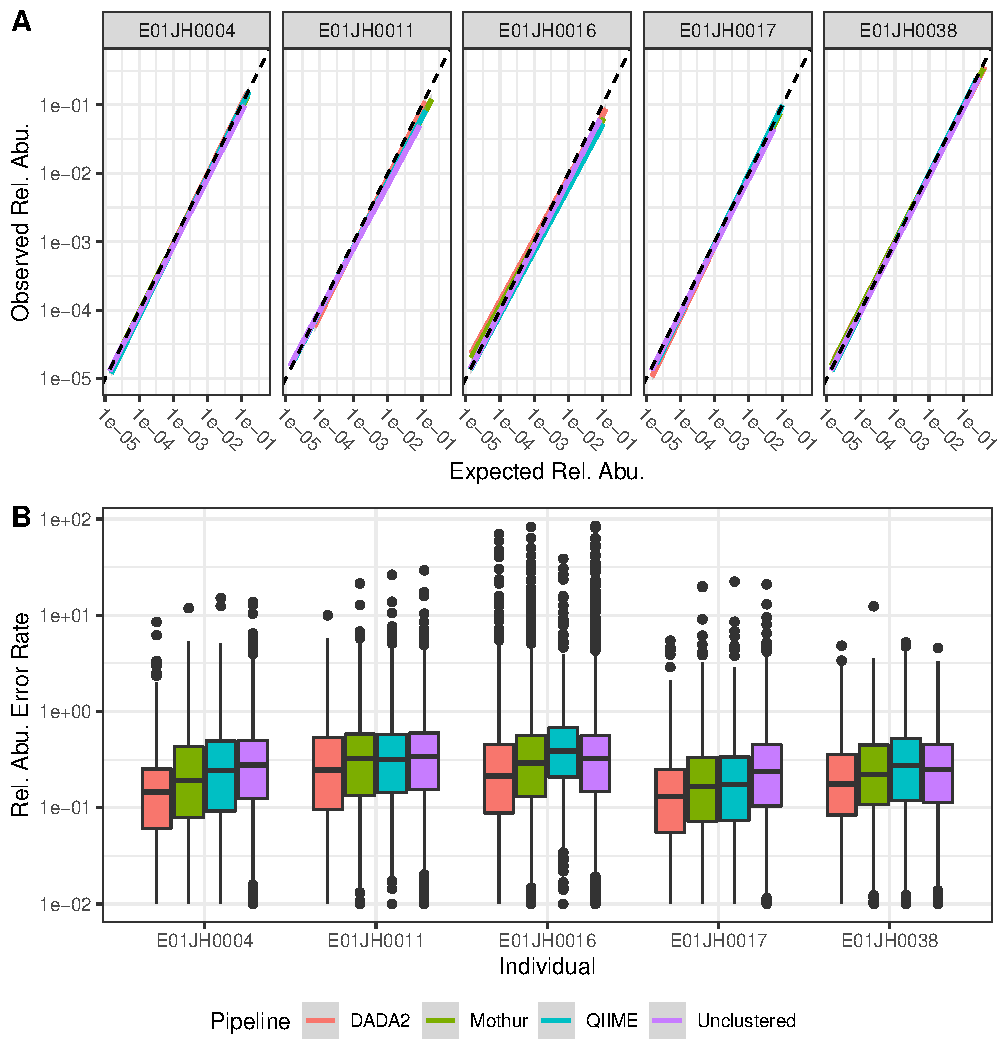
\includegraphics{relAbuError-1.pdf}
\caption{\label{fig:relAbuError}Relative abundance assessment. (A) A linear model of the relationship between the expected and observed relative
abundance. The dashed grey line indicates expected 1-to-1 relationship.
The plot is split by individual and bioinformatic pipeline indicated by line color. A negative binomial model was used to
calculate an average relative abundance estimate across PCR
replicates. To highlight quantitative performance for higher abundance features, points with observed and expected relative abundance values less than 1/median(total abundance) were excluded from the plot.
(B) Relative abundance error rate (\(|expected - observed|/expected\)) distribution by individual and pipeline.}
\end{figure}

\begin{figure}
\centering
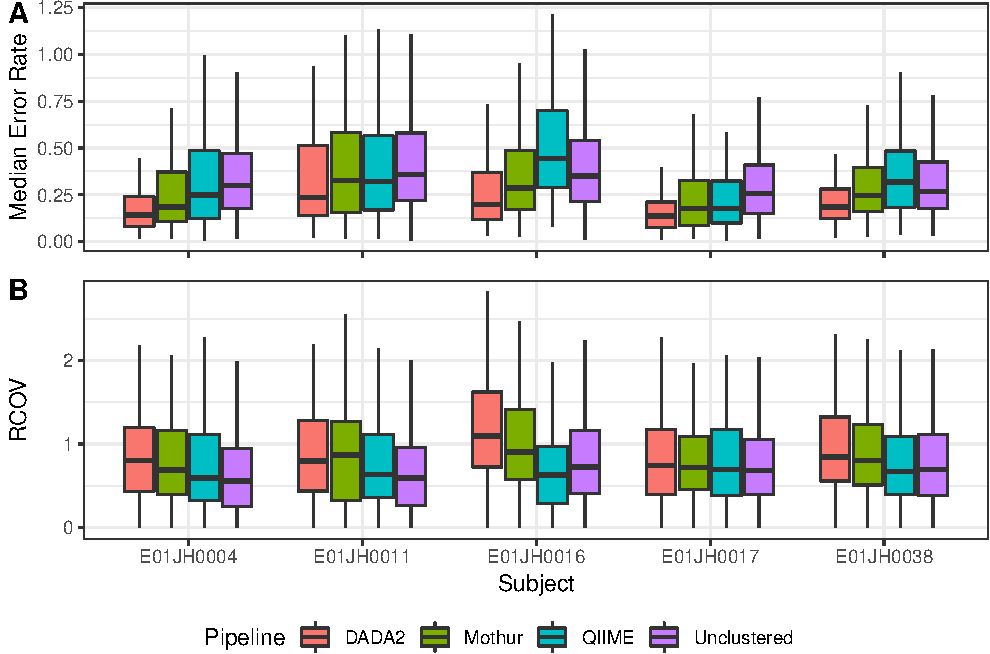
\includegraphics{relAbuErrorMetrics-1.pdf}
\caption{\label{fig:relAbuErrorMetrics}Comparison of pipeline relative
abundance assessment feature-level error metrics. Distribution of
feature-level relative abundance (A) bias metric - median error rate and
(B) variance - robust coefficient of variation (\(RCOV=IQR/|median error rate|\)) by individual and pipeline.
For both the bias and variance metrics lower values are better.
Boxplot outliers, \(1.5\times IQR\) from the median were excluded from the figure to prevent extreme metric values
from obscuring metric value visual comparisons.}
\end{figure}

\begin{table}
\caption{\label{tab:relAbuErrorTbl}Maximum feature-level error rate bias (median error rate) and variance (robust COV) by pipeline and individual.}
\centering
\resizebox{\linewidth}{!}{
\begin{tabular}[t]{llrrrrr}
\toprule
Metric & Pipeline & E01JH0004 & E01JH0011 & E01JH0016 & E01JH0017 & E01JH0038\\
\midrule
 & DADA2 & 2.37 & 2.55 & 17.03 & 4.34 & 0.66\\
\cmidrule{2-7}
 & Mothur & 5.30 & 6.76 & 19.24 & 4.15 & 1.93\\
\cmidrule{2-7}
 & QIIME & 3.99 & 6.43 & 8.83 & 4.80 & 1.09\\
\cmidrule{2-7}
\multirow{-4}{*}{\raggedright\arraybackslash Bias} & Unclustered & 6.45 & 7.24 & 16.85 & 4.37 & 1.91\\
\cmidrule{1-7}
 & DADA2 & 4.60 & 8.96 & 7.36 & 5.91 & 6.71\\
\cmidrule{2-7}
 & Mothur & 4.71 & 7.35 & 3.71 & 5.70 & 8.01\\
\cmidrule{2-7}
 & QIIME & 4.40 & 22.57 & 4.46 & 17.10 & 7.91\\
\cmidrule{2-7}
\multirow{-4}{*}{\raggedright\arraybackslash Variance} & Unclustered & 7.06 & 10.30 & 16.94 & 8.07 & 6.00\\
\bottomrule
\end{tabular}}
\end{table}

\paragraph{Relative Abundance Assessment}
%% Motivation statement
We evaluated the consistency of
the observed and expected relative abundance estimates for a feature and
titration as well as feature-level bias and variance.
Only features observed in all PRE and POST PCR replicates
and PRE and POST specific features were included in the analysis (Table
\ref{tab:relAbuErrorTbl}). Overall, agreement between inferred
and observed relative abundance was high for all individuals and
bioinformatic pipelines (Fig. \ref{fig:relAbuError}A). The error rate
distribution was similarly consistent across pipelines, including long
tails (Fig. \ref{fig:relAbuError}B).

To assess quantitative accuracy we compared the feature-level relative
abundance error rate bias and variance across pipelines and individuals
using mixed effects models. Large bias and variance metric values were
observed for all pipelines (Table \ref{tab:relAbuErrorTbl}). Feature-level relative abundance error rate bias (median error rate, Fig.
\ref{fig:relAbuErrorMetrics}A) was significant different between pipeline but not statistically significant differences was observed for the variance metric, (\(RCOV=(IQR)/|median|\), Fig. \ref{fig:relAbuErrorMetrics}B) across pipeline. The Mothur, DADA2, and QIIME feature-level biases were all significantly different from each other (\(p < 1\times 10^{-8}\)). DADA2 had the lowest mean feature-level bias (0.2), followed by Mothur (0.28), with QIIME having the highest bias
(0.33) (\ref{fig:relAbuErrorMetrics}B). Large variance metric values
were observed for all individuals and pipelines (Table
\ref{tab:relAbuErrorTbl}). The feature-level variance was not
significantly different between pipelines: Mothur = 0.83, QIIME = 0.71
and DADA2 = 1 (Fig. \ref{fig:relAbuErrorMetrics}B).

\paragraph{Differential Abundance Assessment}
\begin{figure}
\centering
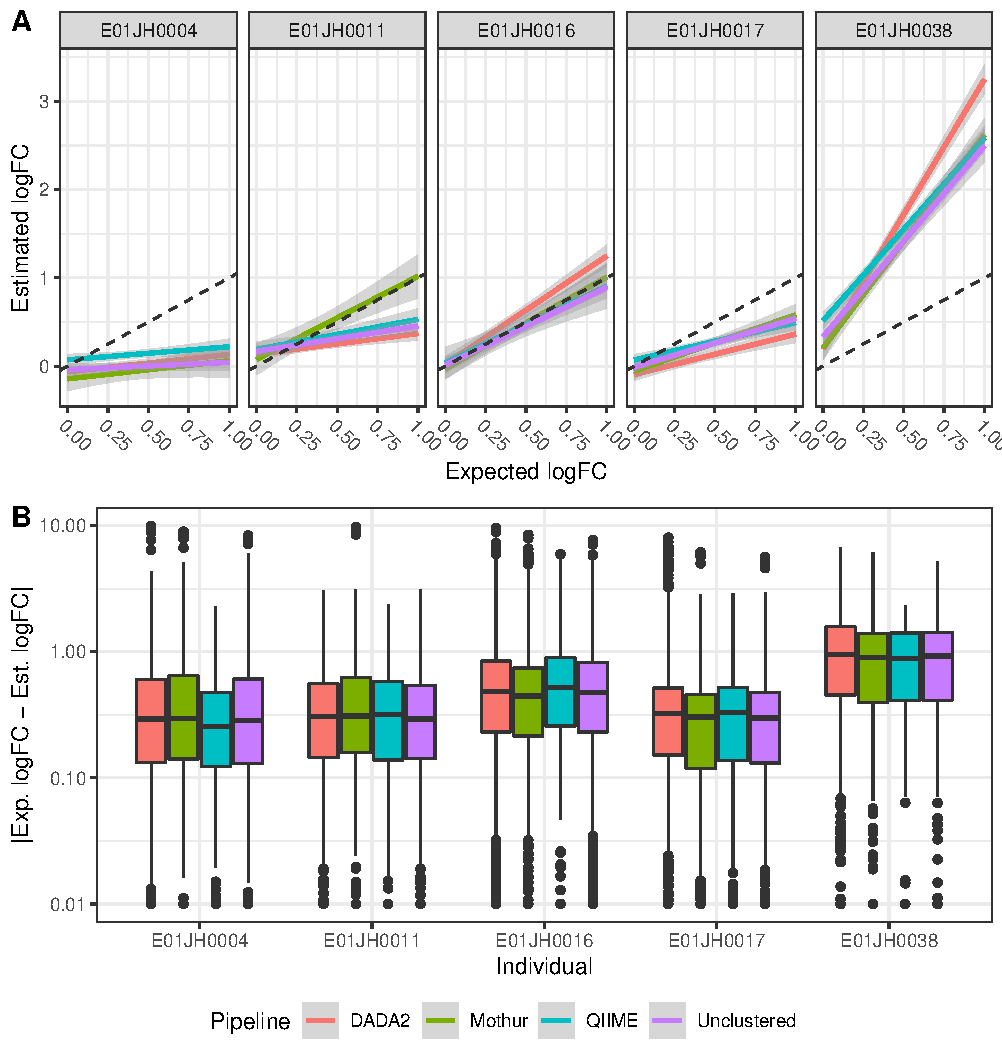
\includegraphics{logFCerror-1.pdf}
\caption{\label{fig:logFCerror} Differential abundance quantitative assessment. (A) Linear model of the relationship between
estimated and expected log fold-change relative abundance between titrations for PRE-specific and
PRE-dominant features by pipeline and individual, line color indicates
pipelines. Dashed grey line indicates expected 1-to-1 relationship
between the estimated and expected log fold-change. (B) Log fold-change
error (\textbar{}exp-est\textbar{}) distribution by pipeline and
individual.}
\end{figure}

\begin{figure}
\centering
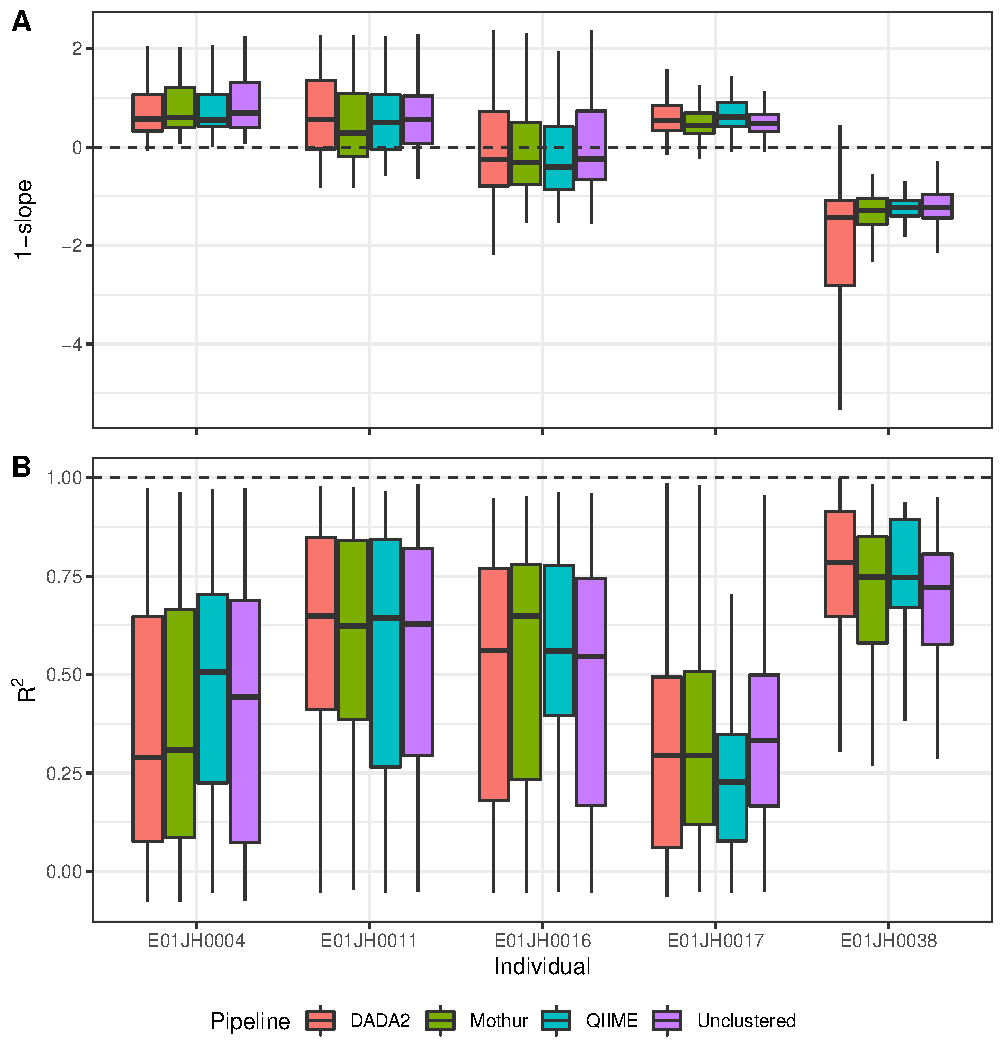
\includegraphics{logFcErrorMetrics-1.pdf}
\caption{\label{fig:logFcErrorMetrics}Feature-level differential abundance assessment. Log-fold change error
bias (A) and variance (B) metric distribution by subject and pipeline.
The bias (\(1 - slope\)) and variance (\(R^2\)) metrics are derived from
the linear model fit to the estimated and expected log fold-change
values for individual features. Boxplot outliers, \(1.5\times IQR\) from
the median were excluded from the figure to prevent extreme metric
values from obscuring metric value visual comparisons.}
\end{figure}

%% Move to discussion?
The agreement between log-fold change estimates and expected values were
individual specific and consistent across pipelines (Fig.
\ref{fig:logFCerror}A). The individual specific effect was attributed to
the fact that unlike relative abundance assessment, the inferred
\(\theta\) values were not used to calculate expected values. Inferred
\(\theta\) values were not used to calculate the expected values because
all of the titrations and the \(\theta\) estimates for the higher
titrations were not monotonically decreasing.
Using the inferred \(\theta\) resulted in unrealistic expected log fold-change values, e.g.,
negative log-fold changes for PRE specific features. The log-fold change
estimates and expected values were consistent across pipelines with one
notable exception. For subject E01JH0011 the Mothur log fold-change estimates
were more consistent with expected values than the other pipelines.
However, as \(\theta\) was not corrected for differences in the
proportion of prokaryotic DNA between the unmixed PRE and POST samples,
it cannot be said whether Mothur's performance was better than the other
pipelines.


The log fold-change error distribution was consistent across pipelines
(Fig. \ref{fig:logFCerror}B). There was a long tail of high error
features in the error distribution for all pipelines and individuals.
The log fold-change estimates responsible for the long tail could not be
attributed to specific titration comparisons. Additionally, we compared
error distributions for log-fold change estimates using
different normalization methods. Error rate distributions, including the
long tails, were consistent across normalization methods. Furthermore,
as the long tail was observed for the unclustered data as well, the
log-fold change estimates contributing to the long tail are likely due
to a bias associated with the molecular portion of the
measurement process and not the computational portion. Exploratory
analysis of the relationship between the log fold-change estimates and
expected values for individual features indicated that the long tails
were attributed to feature specific performance.

Feature-level log fold-change bias and variance metrics were used to
compare pipeline performance (Fig. \ref{fig:logFCerror}). Similar to
relative abundance, feature-level bias and variance metrics are defined
as the \(1 - slope\) and \(R^2\) for linear models of the estimated and
expected log fold-change for individual features and all titration
comparisons. For the bias metric, \(1 - slope\), the desired value is 0
(i.e., log fold-change estimate = log fold-change expected), with
negative values indicating the log-fold change was consistently
underestimated and positive values consistently overestimated. The
linear model \(R^2\) value was used to characterize the feature-level
log fold-change variance as it indicates consistency between log
fold-change estimates and expected values across titration comparisons.
To compare bias and variance metrics across pipelines, mixed-effects
models were used. The log fold-change bias and variance metrics were not
significantly different between pipelines (Bias: F = 0, 2.51, p = 0.99,
0.08, \ref{fig:logFCerror}B, Variance: F = 47.39, 0.23, p = 0, 0.8, Fig.
\ref{fig:logFCerror}C).


\section*{Discussion}
Mixtures of environmental samples have been used to assess
RNAseq and microarray gene expression measurements \cite{parsons2015using, pine2011adaptable, thompson2005use}. However, this is the
first time mixtures have been used to assess microbiome measurement
methods. Using our mixture dataset, we developed novel methods for
assessing marker-gene-survey computational methods. Our quantitative
assessment allowed for the characterization of relative abundance values
on a dataset with more features and higher dynamic range than mock community assessments.

Using mixtures of environmental samples, expected values for use in assessment can be obtained using information from unmixed samples and how the samples were mixed.
Our mixture dataset follows a
two-sample titration mixture design, where DNA collected from five vaccine trial participants before and
after exposure to pathogenic \emph{Escherichia coli}  was mixed following a \(log_2\) dilution
series (Fig. \ref{fig:countExperimentalDesign}).
Count table qualitative characteristics were assessed using relative abundance information for
features observed only in titrations (titration-specific) and unmixed samples (unmixed-specific) (Fig. \ref{fig:featureDefinitions}).
Statistical tests were applied to test if the absence of unmixed-specific features from titrations or absence of titration-specific features from unmixed samples could be explained by random sampling.
Count tables were quantitatively assessed by comparing observed feature relative abundance and feature differential abundance estimates to expected values.
Quantitative performance was characterized using error rate, feature-level bias, and feature-level variance metrics we developed (Fig. \ref{fig:quantMetrics}).


\subsubsection*{Count Table Assessment Demonstration}
The objective of any pipeline is to differentiate true biological sequences from measurement process artifacts and with accurate abundance estimates.
We used our novel assessment approach to evaluate how well three commonly used bioinformatic pipelines, QIIME, Mothur, and DADA2, meet this objective.
Our qualitative assessment results, when combined with sparsity information provides a new method for evaluating how well bioinformatic pipelines account for sequencing artifacts without loss of true biological sequences.
Additionally, our quantitative assessment results identified previously unknown feature specific biases in abundance estimates.

The qualitative assessment evaluates if titration-specific and unmixed-specific features can be explained by random sampling alone (Fig. \ref{fig:featureDefinitions}).
Titration- and unmixed-specific features not explained by sampling are artifacts of the measurement process.
These artifacts can be viewed as false-positives, not representative of actual sequences in a sample, or false-negatives, actual sequences in a sample not represented by count table features.
Count table sparsity information (the proportion of zero-valued cells) can provide additional insight into the qualitative assessment results.

A high false negative rate provides an explanation for DADA2's high proportion of artifact titration- and unmixed-specific features and count table having comparable sparsity to the other pipelines despite having significantly fewer features (Fig. \ref{fig:qualPlot} and Table \ref{tab:pipeQA}).
The DADA2 feature inference algorithm may be aggressively grouping lower abundance true sequences with higher abundance sequences.
As a result, the low abundance sequences are not present in samples leading to increased sparsity and higher abundance unmixed- and titration-specific features.
This aggressive grouping of sequences is a design choice made by the algorithm developers.
The DADA2 documentation states that the default setting for \texttt{OMEGA\_A} is conservative to prevent false positives at the cost of increasing false negatives \cite{callahan2016dada2}.
Using the qualitative assessment methods described here a users can adjust the \texttt{OMEGA\_A} parameter to obtain a false-negative rate appropriate for their study.

While the relative abundance bias metric was significantly different
between pipelines overall, pipeline choice had minimal impact on the
quantitative assessment results when accounting for subject-specific deviations in the proportion of prokaryotic DNA from PRE and POST samples in a titration from the mixture design. Outlier features (those with extreme quantitative analysis bias
and variance metrics) were observed for all pipelines and both abundance assessments.

Outlier features could not be attributed to bioinformatic pipelines and are likely due to biases in the molecular biology part of the measurement process.
Outlier features are unlikely pipeline artifacts as they were observed in count tables generated
using the unclustered pipeline as well as standard bioinformatic
pipelines. Additionally, we were unable to attribute outlier features to relative
abundance values, log fold-change between unmixed samples, and sequence
GC content. Furthermore, features with extreme metric values were not limited to any
specific taxonomic group or phylogenetic clade. PCR amplification bias (a well-known source of bias in the molecular biology part of the
measurement process) is one possible explanation for the outlier features \cite{Sze565598}.
Mismatches in the primer binding regions impact PCR efficiency and are a potential cause for poor feature-specific
performance \cite{wright2014exploiting}. Additional research is needed before outlier features are attributed to mismatches in the primer binding regions.

Based on our assessment results we suggest using DADA2 for feature-level abundance analysis, e.g.~differential abundance testing.
While DADA2 performed poorly in our qualitative assessment, the pipeline performed better in the quantitative assessment compared to the other pipelines.
Additionally, the DADA2 poor qualitative assessment results due to false-negative features are unlikely to negatively impact feature-level abundance analysis.
When determining which pipeline to use for a study, users should consider whether minimizing false positives (DADA2) or false negatives (Mothur) is more appropriate for their study objectives.
When a sequencing dataset is processed using DADA2, the user can be more confident that an observed feature represents a member of the microbial community and not a measurement artifact.

\subsubsection*{Using Mixtures to Assess 16S rRNA Sequencing - Lessons Learned}

There are limitations using our mixture dataset. These limitations
includ: Lack of agreement between the proportion of unmixed samples,
titrations, and the mixture design. The number of features used in the
different analysis and range of expected log-fold changes.
These limitations are described below along with
recommendations for addressing them in future studies.

Differences in the proportion of prokaryotic DNA in the samples used to
generate the two-sample titrations series resulted in differences
between the true mixture proportions and mixture design. We attempted to
account for differences in mixture proportion from mixture design by
estimating mixture proportions using sequence data similar to how the
proportion of mRNA in RNA samples was used in a previous mixture study
\cite{parsons2015using}. We used an assay targeting the 16S rRNA gene
to detect changes in the concentration of prokaryotic DNA across
titrations, but were unable to quantify the proportion of prokaryotic
DNA in the unmixed samples using qPCR data. Using the 16S rRNA sequencing
data, we inferred the proportion of prokaryotic DNA from the POST sample
in each titration. However, the uncertainty and accuracy of the
inference method are not known, resulting in an unaccounted for source of error.

A better method for quantifying sample prokaryotic DNA proportion or
using samples with consistent proportions would increase confidence in
the expected value and in-turn error metric accuracy. Limitations in the
prokaryotic DNA qPCR assay's concentration precision limits the
assay's suitability for use in mixture studies. Digital PCR provides a
more precise alternative to qPCR and is, therefore, a more appropriate
method. Alternatively using samples where the majority of the DNA is
prokaryotic would minimize this issue. Mixtures of environmental samples
can also be used to assess shotgun metagenomic methods as well. As
shotgun metagenomics is not a targeted approach, differences in the
proportion of prokaryotic DNA in a sample would not impact the
assessment results in the same way as 16S rRNA marker-gene-surveys.

Using samples from a vaccine trial allowed for the use of a specific
marker with an expected response, \emph{E. coli}, during methods
development. However, the high level of similarity between the PRE and POST unmixed
samples resulted in a limited number of features that could be used in
the quantitative assessment results. Using more diverse samples to
generate mixtures would address this issue.


\section*{Conclusions}
Our two-sample-titration dataset and assessment methods can be used to evaluate and characterize bioinformatic pipelines and clustering methods.
Count tables produced by any 16S rRNA bioinformatic pipeline can be evaluated using the assessment methods presented here.
Based on out quantitative assessment results for three commonly used bioinformatic pipelines, feature-level results for any 16S rRNA marker-gene survey should be interpreted with care, as the biases responsible for poor quantitative assessment are unknown.
Addressing both of these issues requires advances in both the molecular biology and
computational components of the measurement process.


%%Needs a home - Based on our subject-specific results observation, we recommend that studies using stool samples seeking inferences in a longitudinal series of multiple subjects carefully estimate bacterial DNA proportions and adjust inferences accordingly.



\section*{Methods}
%% Revise to mirror Results structure
\subsection*{Assessment Dataset Development}
ADD INTRO/ TRANSITION TEXT

\subsubsection*{Titration Series Dataset}
ADD INTRO/ TRANSITION TEXT

\paragraph*{Two-Sample Titration Series}
Samples collected at multiple timepoints during a Enterotoxigenic
\emph{E. coli} (ETEC) vaccine trial \cite{harro2011refinement} were
used to generate a two-sample titration dataset for assessing the 16S
rRNA marker-gene survey measurement process. Samples from five trial
participants were selected for our two-sample titration dataset. Trial
participants (subjects) and sampling timepoints were selected based on
\emph{E. coli} abundance data collected using qPCR and 16S rRNA
sequencing from Pop et al. \cite{pop2016individual}. Only individuals with no
\emph{E. coli} detected in samples collected from trial participants
prior to ETEC exposure (PRE) were used for our two-samples titrations.
Post ETEC exposure (POST) samples were identified as the timepoint after
exposure to ETEC with the highest \emph{E. coli} concentration for each
subject (Fig. \ref{fig:countExperimentalDesign}A). Due to limited sample
availability, for E01JH0016 the timepoint with the second highest
\emph{E. coli} concentration was used as the POST sample. Independent
titration series were generated for each subject. POST samples
were titrated into PRE samples with POST proportions of 1/2, 1/4, 1/8,
1/16, 1/32, 1/1,024, and 1/32,768 (Fig.
\ref{fig:countExperimentalDesign}B). Unmixed (PRE and POST) sample DNA
concentration was measured using NanoDrop ND-1000 (Thermo Fisher
Scientific Inc.~Waltham, MA USA). Unmixed samples were diluted to 12.5
\(ng/\mu L\) in tris-EDTA buffer before mixing. The resulting titration series was composed of 45 samples, seven titrations and two unmixed samples for each of the five subjects.


\paragraph*{Sequencing}
The 45 samples were processed using the Illumina 16S library protocol
(16S Metagenomic Sequencing Library Preparation, posted date 11/27/2013,
downloaded from \url{https://support.illumina.com}). This protocol
specifies an initial PCR of the 16S rRNA gene, followed by a sample indexing
PCR, sample concentration normalization, and sequencing.

A total of 192 16S rRNA PCR assays were sequenced across two 96-well plates including four PCR replicates
per sample and 12 no-template controls. The initial
PCR assay targeted the V3-V5 region of the 16S rRNA gene, Bakt\_341F and
Bakt\_806R \cite{klindworth2012evaluation}. The V3-V5 region is 464
base pairs (bp) long, with forward and reverse reads overlapping by 136
bp, using 2 X 300 bp paired-end sequencing \cite{yang2016sensitivity} (
\url{http://probebase.csb.univie.ac.at}). Primer sequences include
overhang adapter sequences for library preparation (forward primer 5'-
TCG TCG GCA GCG TCA GAT GTG TAT AAG AGA CAG CCT ACG GGN GGC WGC AG - 3'
and reverse primer 5'- GTC TCG TGG GCT CGG AGA TGT GTA TAA GAG ACA GGA
CTA CHV GGG TAT CTA ATC C - 3'). Kapa HiFi HotStart
ReadyMix reagents (KAPA Biosystems, Inc.~Wilmington, MA) was used to PCR the 16S rRNA gene. The PCR product amplicon size
was verified using agarose gel electrophoresis.
Concentration measurements were made after the initial 16S rRNA PCR, the
indexing PCR, and normalization steps. DNA concentration was measured
using the QuantIT Picogreen dsDNA Kit (Cat \# P7589, ThermoFisher
Scientific) and fluorescent measurements were made with a Synergy2
Multi-Detection MicroPlate Reader (BioTek Instruments, Inc, Winooski,
VT).

Initial PCR products were purified using 0.8X AMPure XP beads (Beckman
Coulter Genomics, Danvers, MA) following the manufacturer's protocol.
After purification, the 192 samples were indexed using the Illumina
Nextera XT index kits A and D (Illumina Inc., San Diego CA) and then
purified using 1.12X AMPure XP beads. Prior to pooling purified sample
concentration was normalized using SequalPrep Normalization Plate Kit
(Catalog n. A10510-01, Invitrogen Corp., Carlsbad, CA), according to the
manufacturer's protocol. Pooled library concentration was checked using
the Qubit dsDNA HS Assay Kit (Part\# Q32851, Lot\# 1735902,
ThermoFisher, Waltham, MA USA). Due to the low pooled amplicon library
DNA concentration, a modified protocol for low concentration libraries
was used. The library was run on an Illumina MiSeq, and base calls were
made using Illumina Real Time Analysis Software version 1.18.54.
The sequence data was deposited in the NCBI SRA archive under Bioproject
PRJNA480312. Individual SRA run accession numbers and metadata in Supplemental Table.

Sequencing data quality control metrics for the 384 fastq sequence files
(192 samples with forward and reverse reads) were computed using the
Bioconductor \texttt{Rqc} package \cite{Rqc, Bioconductor}.


ADD TEXT??

\paragraph*{Bioinformatic Pipelines}

Sequence data were processed using four bioinformatic pipelines: a
\emph{de-novo} clustering method - Mothur
\cite{schloss2009introducing}, an open-reference clustering method -
QIIME \cite{Caporaso2010}, and a sequence inference method - DADA2
\cite{callahan2016dada2}, and unclustered sequences as a control. The
code used to run the bioinformatic pipelines is available at
\url{https://github.com/nate-d-olson/mgtst_pipelines}.

The Mothur pipeline follows the developer's MiSeq SOP
\cite{schloss2009introducing, kozich2013development}. The pipeline was
run using Mothur version 1.37 (\url{http://www.mothur.org/}). We
sequenced a larger 16S rRNA region, with smaller overlap between the
forward and reverse reads, than the 16S rRNA region the SOP was
designed. Pipeline parameters modified to account for difference in
overlap are noted for individual steps below. The Makefile and scripts
used to run the Mothur pipeline are available
\url{https://github.com/nate-d-olson/mgtst_pipelines/blob/master/code/mothur}.
The Mothur pipeline includes an initial preprocessing step where the
forward and reverse reads are trimmed and filtered using base quality
scores and were merged into single contigs for each read pair. The
following parameters were used for the initial contig filtering, no
ambiguous bases, max contig length of 500 bp, and max homopolymer length
of 8 bases. For the initial read filtering and merging step, low-quality
reads were identified and filtered from the dataset based on the
presence of ambiguous bases, failure to align to the SILVA reference
database (V119, \url{https://www.arb-silva.de/}) \cite{quast2012silva},
and identification as chimeras. Prior to alignment, the SILVA reference
multiple sequence alignment was trimmed to the V3-V5 region, positions
6,388 and 25,316. Chimera filtering was performed using UChime (version
v4.2.40) without a reference database \cite{edgar2011uchime}. OTU
clustering was performed using the OptiClust algorithm with a clustering
threshold of 0.97 \cite{westcott2017opticlust}. The RDP classifier
implemented in Mothur was used for taxonomic classification against the
Mothur provided version of the RDP v9 training set
\cite{wang2007naive}.

The QIIME open-reference clustering pipeline for paired-end Illumina
data was performed according to the online tutorial (Illumina Overview
Tutorial (an IPython Notebook): open reference OTU picking and core
diversity analyses, \url{http://qiime.org/tutorials/}) using QIIME
version 1.9.1 \cite{Caporaso2010}. Briefly, the QIIME pipeline uses
fastq-join (version 1.3.1) to merge paired-end reads
\cite{aronesty2011ea} and the Usearch algorithm \cite{edgar2010search}
with Greengenes database version 13.8 with a 97\% similarity threshold
\cite{desantis2006greengenes} was used for open-reference clustering.

DADA2, an R native pipeline was also used to process the sequencing data
\cite{callahan2016dada2}. The pipeline includes a sequence inference
step and taxonomic classification using the DADA2 implementation of the
RDP naïve Bayesian classifier \cite{wang2007naive} and the SILVA
database V123 provided by the DADA2 developers
\cite[\url{https://benjjneb.github.io/dada2/training.html}]{quast2012silva}.

The unclustered pipeline was based on the Mothur \emph{de-novo}
clustering pipeline, where the paired-end reads were merged, filtered,
and then dereplicated. Reads were aligned to the reference Silva
alignment (V119, \url{https://www.arb-silva.de/}), and reads failing
alignment were excluded from the dataset. Taxonomic classification of
the unclustered sequences was performed using the same RDP classifier
implemented in Mothur used for the \emph{de-novo} pipeline. To limit the
size of the dataset the most abundant 40,000 OTUs (comparable to the
Mothur dataset), across all samples, were used as the unclustered
dataset.

\subsubsection*{Titration Series Validation and Correction}
ADD TEXT

\paragraph*{Volumetric Mixing Validation}


qPCR was used to validate volumetric mixing and check for differences in
the proportion of prokaryotic DNA across titrations
(Fig. \ref{fig:titrationValidation}). To ensure the two-sample titrations
were volumetrically mixed according to the mixture design,
independent ERCC plasmids were spiked into the unmixed PRE and
POST samples \cite{baker2005external} (NIST SRM SRM 2374) (Table
\ref{tab:erccTable}). The ERCC plasmids were resuspended in 100
\(\mu L\) tris-EDTA buffer and 2 \(\mu L\) of resuspended plasmids was
spiked into the appropriate unmixed sample. Plasmids were spiked into
unmixed PRE and POST samples with normalized DNA concentration of
12.5 \(ng/\mu L\). POST sample ERCC plasmid abundance was quantified
using TaqMan gene expression assays (FAM-MGB, Catalog \# 4448892,
ThermoFisher) specific to each ERCC plasmid and TaqMan Universal
MasterMix II (Catalog \# 4440040, ThermoFisher Waltham, MA USA).
qPCR assays were perfomed in triplicate using the QuantStudio
Real-Time qPCR (ThermoFisher). ERCCs were also spiked into PRE
samples but were not used to validate volumetric mixing as PRE sample
proportion differences were too small for qPCR quantification.
The expected difference for the entire range of PRE concentrations
is 1 \(C_t\).

\paragraph*{Prokaryotic DNA Proportion Validation}
To check for differences in the proportion of bacterial DNA in the PRE
and POST samples, bacterial DNA concentration in the titrations was quantified
using the Femto Bacterial DNA quantification kit (Zymo Research, Irvine
CA). All samples were run in triplicate along with an in-house \emph{E.
coli} DNA \(log_{10}\) dilution standard curve. Three concentrations were used
for the in-house standard, 20 ng/ul, 2ng/ul, and 0.2 ng/ul,
with 91.49 efficiency and 0.999 \(R^2\). qPCR assays were
performed using the QuantStudio Real-Time qPCR (ThermoFisher).
Amplification data and Ct values were exported as tsv files using
QuantStudio™ Design and Analysis Software v1.4.1. Statistical analysis
was performed on the exported data using custom scripts in R \cite{R}.
The qPCR data and scripts used to analyze the data are available at
\url{https://github.com/nate-d-olson/mgtst_pub}.

\paragraph*{Correcting for Deviations from Mixture Design}
The following linear model \eqref{eq:thetaInf} was used to infer the
proportion of prokaryotic DNA, \(\theta\), in each titration. Where
\(\textbf{Q}_{i}\) is a vector of titration \(i\) feature relative
abundance estimates and \(\textbf{Q}_{pre}\) and \(\textbf{Q}_{post}\)
are vectors of feature relative abundance estimates for the unmixed PRE
and POST samples. Feature relative abundance estimates were calculated
using a negative binomial model.

\begin{equation}
  \textbf{Q}_{i} = \theta_i (\textbf{Q}_{post} -\textbf{Q}_{pre}) + \textbf{Q}_{pre}
  \label{eq:thetaInf}
\end{equation}

To fit the model and prevent uninformative and low abundance features
from biasing \(\theta\) estimates, only features meeting the following
criteria were used. To improve feature level model fit, features had to be observed in at least 14 of the 28 total titration PCR replicates (4 replicates per 7 titrations.)
To increase confidence in PRE and POST abundance estimates the features were present in either all four or none of the PRE and POST PCR replicates.
Finally, to eliminate uninformative features with no change in abundance across titrations only features with greater than 2-fold difference in relative abundance between the PRE and POST samples were used.

16S rRNA sequencing count data is known to have a non-normal
mean-variance relationship resulting in poor model fit for standard
linear regression \cite{McMurdie2014}. Generalized linear models
provide an alternative to standard least-squares regression. The above
model is additive and therefore \(\theta_i\) cannot be directly inferred
in log-space. To address this limitation, we fit a model to \eqref{eq:thetaInf}
using standard least-squares regression and obtained non-parametric 95 \%
confidence intervals for the \(\theta\) estimates by bootstrapping with 1000
replicates. Bootstrapping was performed by resampling informative features, defined above, by subject.

\subsection*{Assessment Framework}
To assess the qualitative and quantitative performance of marker-gene survey analysis methods we developed a framework utilizing our two-sample titration dataset. Qualitative assessment evaluates feature presence-absence. The quantitative assessment evaluates the relative and differential abundance estimates.

\subsubsection*{Qualitative Assessment}
\paragraph*{Artifactual Feature Proportion}

Our qualitative measurement assessment evaluated features only observed
in unmixed samples (PRE or POST), \emph{unmixed-specific}, or
titrations, \emph{titration-specific} (Fig.
\ref{fig:featureDefinitions}. \emph{Unmixed-} or
\emph{titration-specific} features are due to differences in sampling
depth (number of sequences) between the unmixed samples and titrations,
artifacts of the feature inference process, or PCR/sequencing artifacts.
Measurement process artifacts should be considered false positives or
negatives. Hypothesis tests were used to determine if differences in
sampling depth could account for \emph{unmixed-specific} and
\emph{titration-specific} features. p-values were adjusted for multiple
comparisons using the Benjamini \& Hochberg method
\cite{benjamini1995controlling}. For \emph{unmixed-specific} features,
the binomial test was used to evaluate if true feature relative
abundance is less than the expected relative abundance. A binomial test
could not be used to evaluate \emph{titration-specific} features, as the
hypothesis would be formulated as such. Given observed counts and the
titration total feature abundance, the true feature relative abundance
is equal to 0. As non-zero counts were observed, the true feature
proportion is non-zero, and the test always fails. Therefore, we
formulated a Bayesian hypothesis test for \emph{titration-specific}
features.

The Bayesian hypothesis test evaluated if the true feature
proportion is less than the minimum detected proportion. The Bayesian
hypothesis test was formulated using equation \eqref{eq:bht}. Which, when
assuming equal priors, \(P(\pi < \pi_{min}) = P(\pi \geq \pi_{min})\),
reduces to \eqref{eq:bht2}. For equations \eqref{eq:bht} and \eqref{eq:bht2}
\(\pi\) is the true feature proportion, \(\pi_{min}\) is the minimum
detected proportion, \(C\) is the expected feature counts, and
\(C_{obs}\) is the observed feature counts. Simulation was used to
generate possible values of \(C\), assuming \(C\) has a binomial
distribution given the observed sample total feature abundance, and a
uniform probability distribution for \(\pi\) between 0 and 1.
\(\pi_{min}\) was calculated using the mixture equation \eqref{eq:mixEq}
where \(q_{pre,j}\) and \(q_{post,j}\) are \(min(\textbf{Q}_{pre})\) and
\(min(\textbf{Q}_{post})\) across all features for a subject and
pipeline. Our assumption is that \(\pi\) is less than \(\pi_{min}\) for
features not observed in unmixed samples due to random sampling.

\begin{equation}
  \begin{split}
    p & = P(\pi < \pi_{min} | C \geq C_{obs}) \\
      & = \frac{P(C \geq C_{obs}| \pi < \pi_{min})P(\pi < \pi_{min})}{P(C \geq C_{obs}| \pi < \pi_{exp})P(\pi < \pi_{min}) + P(C \geq C_{obs}| \pi \geq \pi_{min})P(\pi \geq \pi_{min})} \\
  \end{split}
  \label{eq:bht}
\end{equation}

\begin{equation}
p = \frac{P(C \geq C_{obs}| \pi < \pi_{min})}{P(C \geq C_{obs})}
  \label{eq:bht2}
\end{equation}

\paragraph*{Sparsity}
ADD TEXT


\subsubsection*{Quantitative Assessment}
For quantitative assessment, we compared observed relative abundance and
log fold-changes to expected values derived from the titration
experimental design.

\paragraph*{Relative Abundance Assessment}

Feature average relative abundance across PCR
replicates was calculated using a negative binomial model, and used as
observed relative abundance values (\(obs\)) for the relative abundance
assessment. Average relative abundance values were used to reduce PCR
replicate outliers from biasing the assessment results. Equation
\eqref{eq:mixEq} and inferred \(\theta\) values were used to calculate the
expected relative abundance values (\(exp\)). Relative abundance error
rate is defined as \(|exp - obs|/exp\).
We developed bias and variance metrics to assess feature performance.
The feature-level bias and variance metrics were defined as the median
error rate and robust coefficient of variation (\(RCOV=IQR/median\))
respectively. Mixed-effects models were used to compare feature-level
error rate bias and variance metrics across pipelines with subject as a
random effect. Extreme feature-level error rate bias and variance metric
outliers were observed, these outliers were excluded from the mixed
effects model to minimize biases due to poor model fit and were
characterized independently.

\paragraph*{Differential Abundance Assessment}

Log fold-change between samples in the titration series including PRE
and POST were compared to the expected log fold-change values to assess
differential abundance log fold-change estimates. Log fold-change
estimates were calculated using EdgeR
\cite{Robinson2010, McCarthy2012}. Expected log fold-change for feature
\(j\) between titrations \(l\) and \(m\) is calculated using equation
\eqref{eq:expLogFC}, where \(\theta\) is the proportion of POST bacterial
DNA in a titration, and \(q\) is feature relative abundance. For
features only present in PRE samples the expected log fold-change is
independent of the observed counts for the unmixed samples and is
calculated using \eqref{eq:expPreLogFC}. Features only observed in POST
samples, \emph{POST-specific}, expected log fold-change values can be
calculated in a similar manner. However, \emph{POST-specific} features
were rarely observed in more than one titration and therefore were not
suitable for use in our assessment. Due to a limited number of
\emph{PRE-specific} features, both \emph{PRE-specific} and
\emph{PRE-dominant} features were used in the differential abundance
assessment. \emph{PRE-specific} features were defined as features
observed in all four PRE PCR replicates and not observed in any of the
POST PCR replicates and \emph{PRE-dominant} features were also observed
in all four PRE PCR replicates and observed in one or more of the POST
PCR replicates with a log fold-change between PRE and POST samples
greater than 5.

\begin{equation}
      logFC_{lm,j} = \log_2\left(\frac{\theta_l q_{post,j} + (1 - \theta_l) q_{pre,i}}{\theta_m q_{post,j} + (1 - \theta_m) q_{pre,j}}\right)
  \label{eq:expLogFC}
\end{equation}

\begin{equation}
      logFC_{lm,i} = log_2\left(\frac{1-\theta_l}{1-\theta_m}\right)
  \label{eq:expPreLogFC}
\end{equation}


\subsection*{Count Table Assessment Demonstration}
Demonstrate framework by comparing the qualitative and quantitative assessment results across the three pipelines.

\subsubsection*{Count Table Characteristics - TODO}
Count tables summarized for
- number of features
- total abundance
- filter rate
- taxonomic composition

\subsubsection*{Qualitative Assessment - TODO}
- comparison of observed and expected abundance for titration- and unmixed-specific features
- compared proportion of titration- and unmixed-specific features with abundance values that could not be explained by sampling alone
- qualitatitve comparison of sparsity values

\subsubsection*{Quantitative Assessment}
Mixed-effects models were used to compare relative and differential abundance bias and variance metric distributions across the three pipelines.

Need to replace with equation or better describe in the text.
\begin{verbatim*}
Example mixed effect model in R

error_fit <- nlme::lme(median_error ~ pipe, random =  ~ 1 | biosample_id, data = error_fit_dat)
\end{verbatim*}

Features with large bias and variance metrics, \(1.5\times IQR\) from the median,
were deemed outliers. To prevent these outlier features from biasing the
comparison, they were not used to fit the mixed effects model. Multiple
comparisons test (Tukey) was used to test for significant differences in
feature-level bias and variance between pipelines. A one-sided
alternative hypothesis was used to determine which pipelines had smaller
feature-level error rate.

Need to replace with equation or better describe in the text.
\begin{verbatim*}
Example post-hoc test in R

error_post_hoc <- glht(error_fit, linfct = mcp(pipe = "Tukey"), alternative = "greater")
\end{verbatim*}



%%%%%%%%%%%%%%%%%%%%%%%%%%%%%%%%%%%%%%%%%%%%%%
%%                                          %%
%% Backmatter begins here                   %%
%%                                          %%
%%%%%%%%%%%%%%%%%%%%%%%%%%%%%%%%%%%%%%%%%%%%%%

\begin{backmatter}

\section*{Declarations}

\subsection*{Ethics approval and consent to participate}
Not applicable.

\subsection*{Consent for publication}
Not applicable.

\subsection*{Availability of data and material}
Sequence data was deposited in the NCBI SRA archive under Bioproject
PRJNA480312.
Individual SRA run accession numbers and metadata in Supplemental Table.
The code used to run the bioinformatic pipelines is available at
\url{https://github.com/nate-d-olson/mgtst_pipelines}.
Scripts used to analyze the data are available at
\url{https://github.com/nate-d-olson/mgtst_pub}.

\subsection*{Competing interests}
The authors declare that they have no competing interests.

\subsection*{Funding}
This work was partially supported by National Institutes of Health (NIH)
{[}NIH R01HG005220 to H.C.B.{]}

\subsection*{Authors' contributions}
NDO, HCB, OCS, MS, and WT designed the experiment, SL and SH performed the laboratory work.
NDO, HCB and MS analyzed the data.
NDO and HCB wrote the manuscript.
All authors provided feedback on manuscript drafts and approved the final manuscript.


\subsection*{Acknowledgements}
 The authors would like to thank Mihai
Pop, Scott Pine, Scott Jackson, Justin Zook, and Prachi Kulkarni for
feedback on manuscript drafts. Opinions expressed in this paper are the
authors and do not necessarily reflect the policies and views of NIST,
or affiliated venues. Certain commercial equipment, instruments, or
materials are identified in this paper in order to specify the
experimental procedure adequately. Such identification is not intended
to imply recommendations or endorsement by NIST, nor is it intended to
imply that the materials or equipment identified are necessarily the
best available for the purpose. Official contribution of NIST; not
subject to copyrights in USA.



%%%%%%%%%%%%%%%%%%%%%%%%%%%%%%%%%%%%%%%%%%%%%%%%%%%%%%%%%%%%%
%%                  The Bibliography                       %%
%%                                                         %%
%%  Bmc_mathpys.bst  will be used to                       %%
%%  create a .BBL file for submission.                     %%
%%  After submission of the .TEX file,                     %%
%%  you will be prompted to submit your .BBL file.         %%
%%                                                         %%
%%                                                         %%
%%  Note that the displayed Bibliography will not          %%
%%  necessarily be rendered by Latex exactly as specified  %%
%%  in the online Instructions for Authors.                %%
%%                                                         %%
%%%%%%%%%%%%%%%%%%%%%%%%%%%%%%%%%%%%%%%%%%%%%%%%%%%%%%%%%%%%%

% if your bibliography is in bibtex format, use those commands:
\bibliographystyle{bmc-mathphys} % Style BST file (bmc-mathphys, vancouver, spbasic).
\bibliography{abundanceAssessment}      % Bibliography file (usually '*.bib' )
% for author-year bibliography (bmc-mathphys or spbasic)
% a) write to bib file (bmc-mathphys only)
% @settings{label, options="nameyear"}
% b) uncomment next line
%\nocite{label}

% or include bibliography directly:
% \begin{thebibliography}
% \bibitem{b1}
% \end{thebibliography}


\end{backmatter}
\end{document}
